
%version 2: \usepackage{hyperref}


%%%%%%%%%%%%%%%%%%%%%%%%%%%%%%%%%%%%%%%%%%%%%%%%%%%%%%%%%%%%%%%%%%%%%%%%
%Para las ecuaciones siempre es Ec.(n).
%Para las figuras siempre es Fig.n, incluso en el caption de la figura. Tambien las Tablas
%Para las referencias es [n]
%%%%%%%%%%%%%%%%%%%%%%%%%%%%%%%%%%%%%%%%%%%%%%%%%%%%%%%%%%%%%%%%%%%%%%%%

\documentclass[
reprint,
%notitlepage,
%superscriptaddress,
%groupedaddress,
%unsortedaddress,
%runinaddress,
%frontmatterverbose, 
%preprint,
%showpacs,preprintnumbers,
%nofootinbib,
%nobibnotes,
%bibnotes,
%11 pt,
amsmath,
amssymb,
%aps,
%pra,
prb,
%rmp,
%tightenlines %esto hizo el milagro de sacar los espacios en blancos estocásticos (?)
%prstab,
%prstper,
%floatfix,\textbf{}
]{revtex4-1} %Instalar primero para usarlo. Paquete malo.

%\documentclass[onecolumn, aps, amsmath,amssymb ]{article}
\usepackage{lipsum}  
\usepackage{graphicx}% Include figure files
\usepackage{subfig}
\usepackage{braket}
\usepackage{comment} %comment large chunks of text
\usepackage{dcolumn}% Align table columns on decimal point
\usepackage{bm}% bold math
%\usepackage{hyperref}% add hypertext capabilities
\usepackage[mathlines]{lineno}% Enable numbering of text and display math
%\linenumbers\relax % Commence numbering lines
\usepackage{mathtools} %% Para el supraíndice

\usepackage[nice]{nicefrac}

%%%%%%%El Señor Español%%%%%%%%%%%%%%%%%%%%%%%%%%%
\usepackage[utf8]{inputenc} %acento
\usepackage[
spanish, %El lenguaje.
es-tabla, %La tabla y no cuadro.
activeacute, %El acento.
es-nodecimaldot %Punto y no coma con separador de números
]{babel}
\usepackage{microtype} %para hacerlo más bonito :33 como vos (?) 
%%%%%%%%%%%%%%%%%%%%%%%%%%%%%%%%%%%%%%%%%%%%%%%%%%%
%%%%%%%%% Para que las imágenes se queden dónde las quiero (?
\usepackage{float}
%%%%%%%%%%
\usepackage{enumitem}
\usepackage{hyperref} % Para usar \url

%%%%%%%%Cambia a Fig de Figure%%%%%%%%%%
\makeatletter
\renewcommand{\fnum@figure}{Fig. \thefigure} 
\makeatother
%%%%%%%%%%%%%%%%%%%%%%%%%%%%%%%%%%%%%%%%
\raggedbottom

\usepackage{multirow}
\begin{document}

\title{Práctica 2: Introducción a las redes neuronales}
\author{Evelyn~G.~Coronel}

\affiliation{
Aprendizaje Profundo y Redes Neuronales Artificiales\\ Instituto Balseiro\\}

\date[]{\lowercase{\today}} 

\maketitle

\section*{Ejercicio 1}

En el ejercicio 1 se calcularon las funciones de activación y sus gradientes para un perceptron con una entrada de dos dimensiones. Debido a la utilización  de bias, definimos $\tilde x = \{ x, 1\}$ y $\tilde w =\{ w, b \}$ a partir de esto:
\begin{itemize}
    \item Entrada: $ \vec x = (2.8, -1.8)$
    \item Pesos: $ \vec w = (1.45, -0.35)$
    \item Bias: $b= -4$
\end{itemize}

Pasamos a los siguiente:
\begin{itemize}
\item Entrada modificada: $ \tilde x = (2.8, -1.8, 1)$
\item Pesos modificados: $\tilde  w = (1.45, -0.35, -4)$.
\end{itemize}
Mientras que el producto entre los pesos y la entrada de la red es la siguiente $y = \sum_i \tilde x_i \tilde{w}_i = 0.69$.

Se calcularon las activaciones (marcados en color azul) y gradientes (marcados en color  verde y rojo) para distintas funciones, siguiendo los siguientes pasos:

\begin{enumerate}
    \item Calculamos $y = \tilde{w} \cdot \tilde{x}$  
    \item Calculamos la salida de la función de activación f(y) (en azul)  y su derivada f'(y) (en verde).
    \item Considerando la tasa de aprendizaje $\eta$, la variación del peso es $\frac{\delta \tilde w_i}{\eta} = \frac{df(y)}{d \tilde w_i} = f'(y) \tilde x_i$ (en rojo)
\end{enumerate}

Los cálculos para cada función de activación se muestran a continuación:

\begin{enumerate}[label=(\alph*)]
    \item Función Sigmoidal:
    
    Los cálculos se muestran en la Fig.\,\ref{fig:1a}, y las funciones son las siguientes:
    \[
        f(x) = \frac{1}{1 + e^{-x}}
    \]
    
    \[
       \text{Derivada: } f'(x) = \frac{e^{-x}}{(1 + e^{-x})^2} =  e^{-x}\times f(x)
    \]

    \item Función de la tangente hiperbólica:
    
    Los cálculos se muestran en la Fig.\,\ref{fig:1b}, y las funciones son las siguientes:
    \[  
        \tanh(x) = \frac{e^{x} - e^{-x} }{e^{x} + e^{-x}}
    \]
    \[
        \text{Derivada: }  f'(x) =  (\cosh{x})^{-2} = 1 - \tanh^2x = 1 - f(x)^2
    \]



    \item Función ELU (Exponential Linear Unit):
    
    Los cálculos se muestran en la Fig.\,\ref{fig:1c}, y las funciones son las siguientes:

    \[  f(x)=
        \begin{cases}
            x  & x \geq 0 \\
            \alpha(e^x - 1) & x < 0\\
        \end{cases}
        \]

    \[  \text{Derivada: } f'(x)=
        \begin{cases}
            1  & x \geq 0 \\
            \alpha e^x & x < 0\\
        \end{cases}
        \]


        \begin{figure}[H]
            \begin{small}
                \begin{center}
                    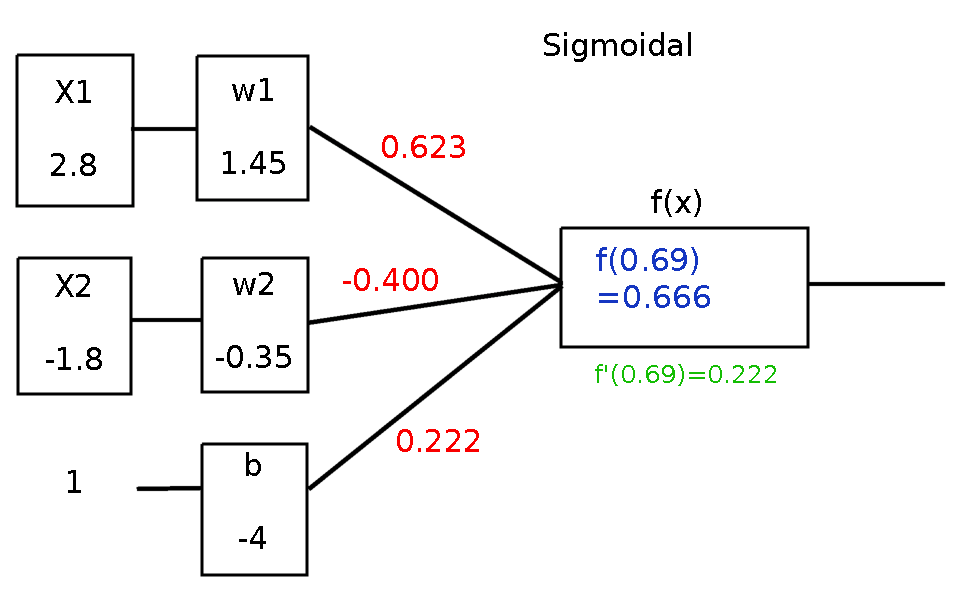
\includegraphics[width=0.5\textwidth]{Graphs/ejer1a.pdf}
                \end{center}
                \caption{Activaciones y gradientes para la función sigmoidal.}
                \label{fig:1a}
            \end{small}
        \end{figure}

        \begin{figure}[H]
            \begin{small}
                \begin{center}
                    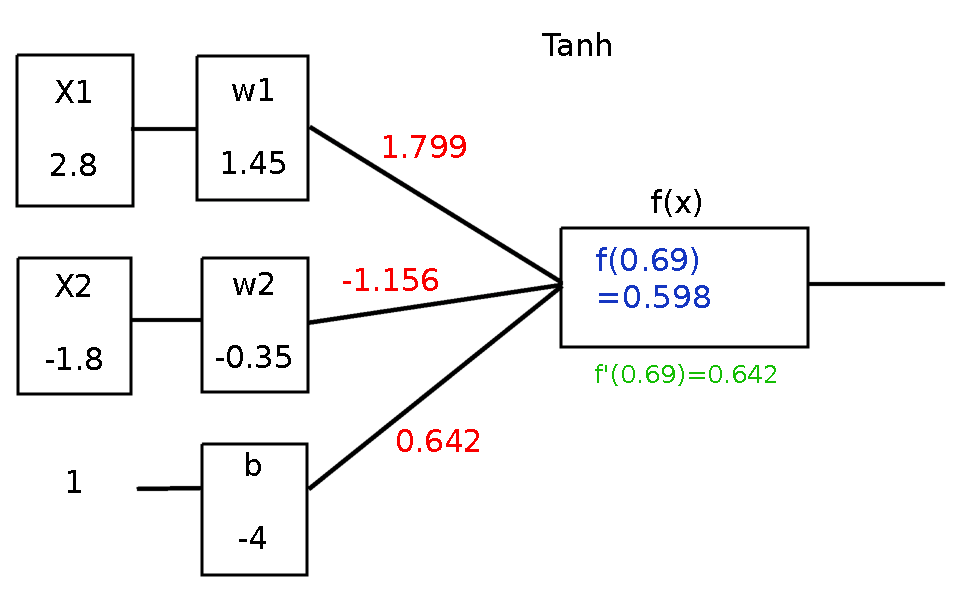
\includegraphics[width=0.5\textwidth]{Graphs/ejer1b.pdf}
                \end{center}
            \caption{Activaciones y gradientes para la función de la tangente hiperbólica.}
            \label{fig:1b}
            \end{small}
        \end{figure}
        

        \begin{figure}[H]
            \begin{small}
                \begin{center}
                    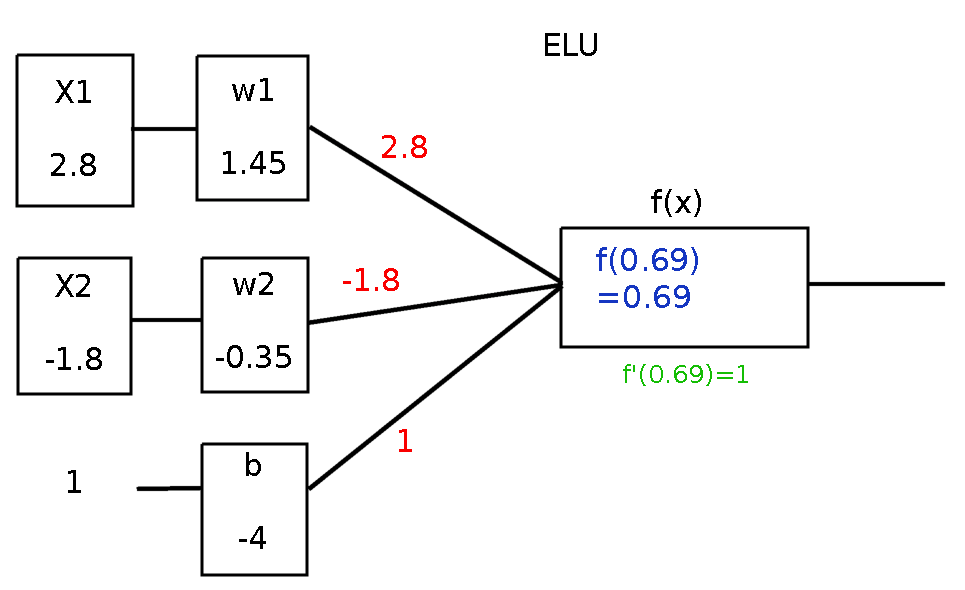
\includegraphics[width=0.5\textwidth]{Graphs/ejer1c.pdf}
                \end{center}
                \caption{Activaciones y gradientes para la función ELU (Exponential Linear Unit).}
                \label{fig:1c}
            \end{small}
        \end{figure}
        

    \item Función Leaky ReLU (Rectified Linear Unit):
    
    Los cálculos se muestran en la Fig.\,\ref{fig:1d}, y las funciones son las siguientes:

    \[ f(x) = max(0.1x, x)  \]
    \[ \text{Derivada: } f'(x) =    \begin{cases}
                    0.1  & x < 0 \\
                    1    & x > 0\\
                 \end{cases}  \]

    \begin{figure}[H]
        \begin{small}
            \begin{center}
                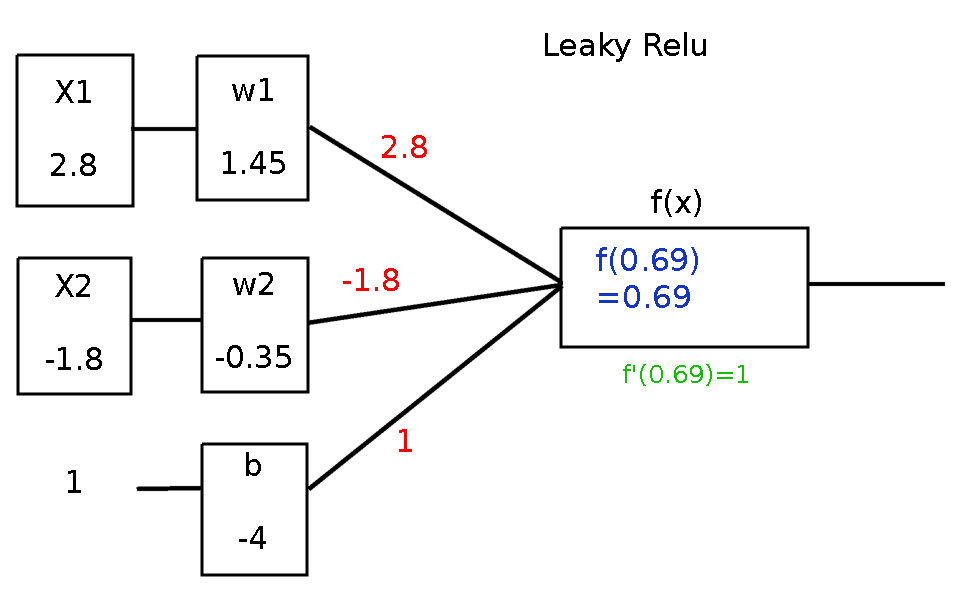
\includegraphics[width=0.5\textwidth]{Graphs/ejer1d.pdf}
            \end{center}
            \caption{Activaciones y gradientes para la función Leaky ReLU (Rectified Linear Unit)}
            \label{fig:1d}
        \end{small}
    \end{figure}

\end{enumerate}

\section*{Ejercicio 2}

En este ejercicio se calcularon las activaciones y gradientes de una arquitectura con datos de entrada bidimensionales, una capa oculta con dos neuronas de activación sigmoidal, y una función de pérdida Mean Square Error (MSE).

Las condiciones de este calculo de activaciones y gradientes son  las siguientes:
\begin{itemize}
    \item Entrada: $x= (-3.1, 1.5)$, con  el bias $x'=(-3.1, 1.5, 1)$
    \item Bias: $b_1=-4$  y $b_2=-1$
    \item Pesos: \[ W=
        \begin{bmatrix}
            -0.2 & 2  \\ 
            -0.5 &-0.3 \\
        \end{bmatrix}
        \]
        Con el bias
        \[ W'=
        \begin{bmatrix}
            -0.2 & 2  & -4\\ 
            -0.5 &-0.3 & -1\\
        \end{bmatrix}
        \]
\end{itemize}

Para realizar los cálculos se siguen los siguientes pasos:

\begin{enumerate}
    \item Se calcula $\vec y = \bf{W} \cdot \vec x + \vec b$, donde $\vec b = (b_1, b_2)$.
    \item El vector $\vec y$ es bidimensional, y se aplica a cada la función de activación a cada componente $f(\vec y)$. (Números en azul).
    \item Calculamos el MSE (en azul) y el gradiente del MSE de la salida (en rojo).
    \item Considerando la tasa de aprendizaje $\eta$,  la variación del peso es
    \[ \frac{\delta W_{ij}}{\eta} = \frac{df(\vec y)}{d W_{ij}} = f'(y_i)\delta_{jm}  x_m \]
    (en rojo). En forma matricial, esto se puede escribir como 
    \[\frac{\delta \bf{W}}{\eta} = \vec x (f'(\vec y))^T\]
\end{enumerate}


\begin{figure}[H]
    \begin{small}
        \begin{center}
            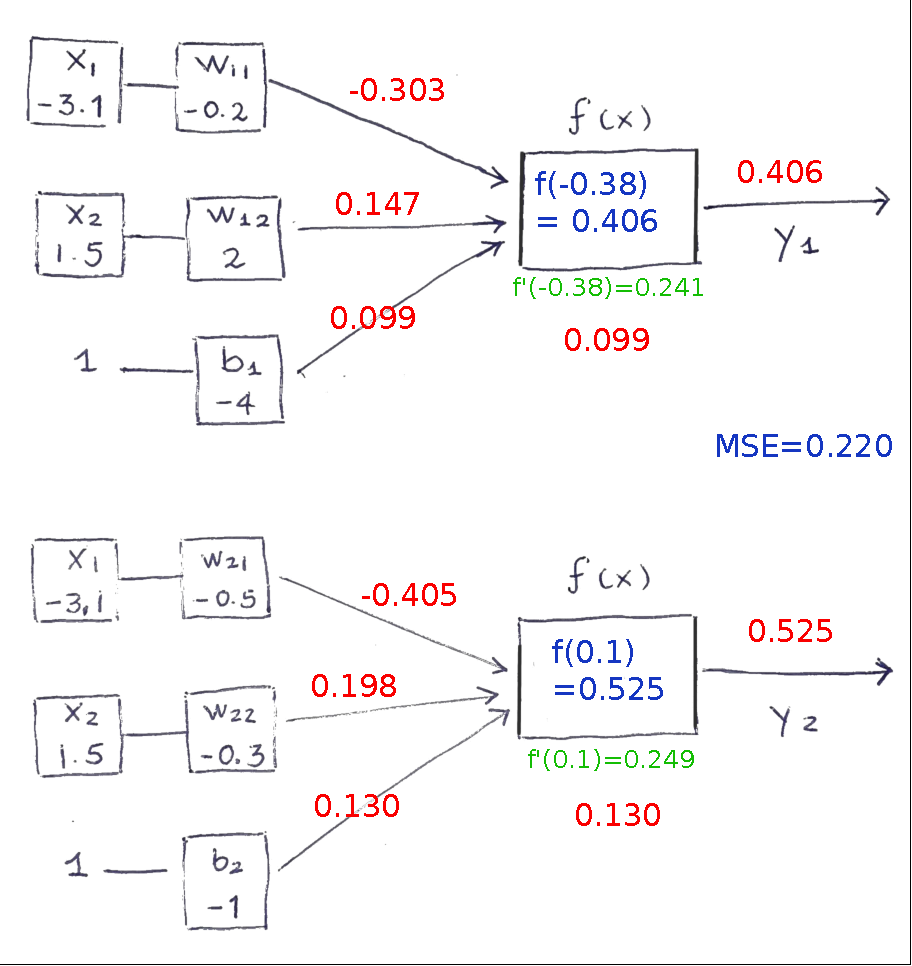
\includegraphics[width=0.482\textwidth]{Graphs/ejer2_grafico.pdf}
        \end{center}
        \caption{Análogo al ejercicio 1, se calcularon las activaciones y los gradientes para la arquitectura mostrada en la figura.}
        \label{fig:}
    \end{small}
\end{figure}

\section*{Clasificando las imágenes del CIFAR-10}


En estos ejercicios se intenta clasificar las imágenes del CIFAR-10 con la siguiente arquitectura:  Entrada con una entrada constante $1$ para el bias, capa oculta de 100 neuronas con bias y la salida. La entrada consiste en las imágenes del CIFAR-10, de tal forma que sea unidimensionales con $3072$ valores y la salida de 10 valores. Las capas están totalmente conectadas y se utilizada el optimizador \emph{Gradiente descendiente por batch}, con un tamaño de batch  de $50$ ejemplos.

En el pre-procesado de los datos de entrenamiento, los mismos se les resta la media del conjunto y se divide por $255$, el máximo valor posible. A los datos de validación se les resta la media del entrenamiento y también se divide por $255$


Las precisiones de la validación obtenidas de estas redes en función de las épocas se comparan con las precisiones obtenidas en con los clasificadores Soft-Max y Support Vector  Machine. Las últimas se calcularon con una tasa de aprendizaje de $0.0002$, con pesos inicializados uniformemente entre  $[-0.0001, 0.0001]$.

\subsection*{Ejercicio 3}
En este caso, las funciones de activación de la capa oculta y de salida son una función sigmoidal y lineal respectivamente,  y la función de pérdida es la MSE. En las Figs.\,\ref{fig:ejer3_acc} y \ref{fig:ejer3_loss} se muestran la precisión y la pérdida, normalizada por el máximo valor, función de las épocas de entrenamiento.

\begin{figure}[H]
    \begin{small}
        \begin{center}
            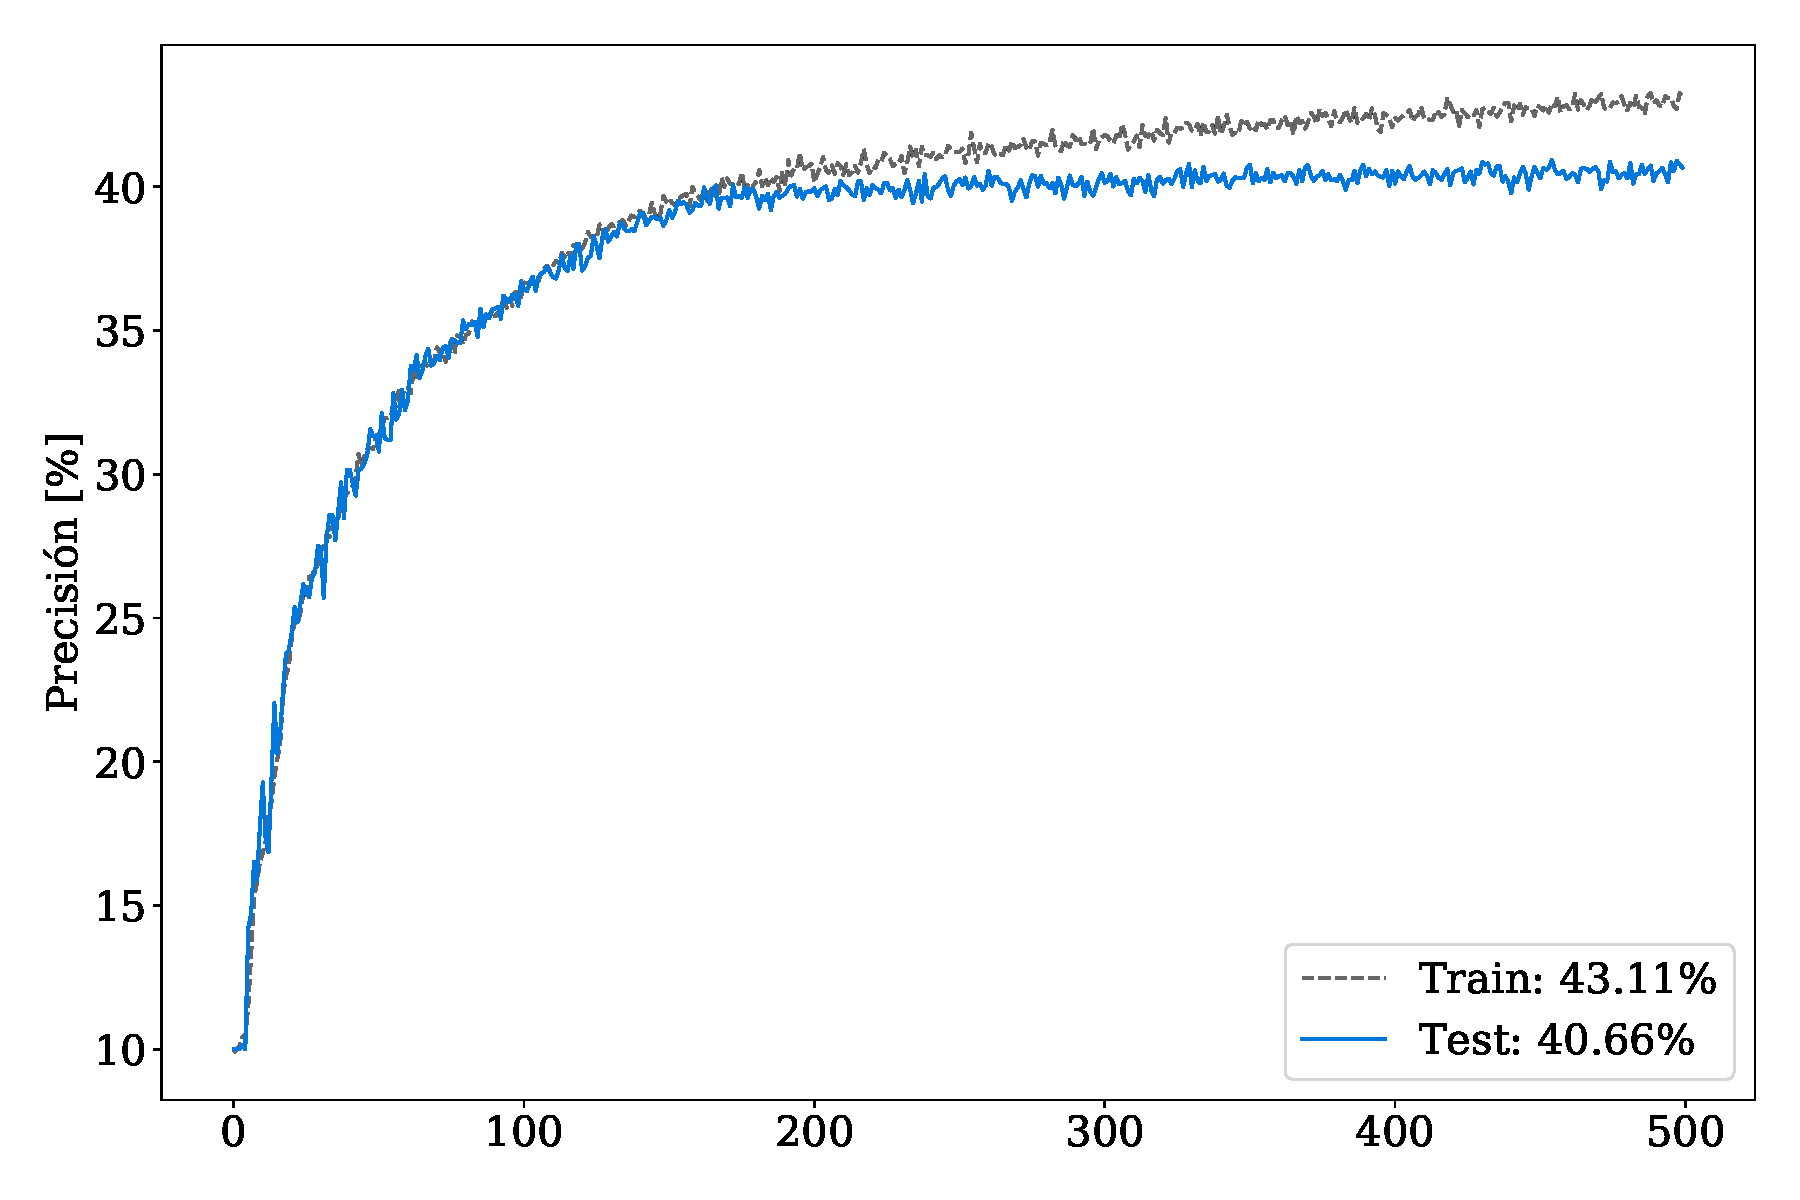
\includegraphics[width=0.495\textwidth]{Graphs/ejer3_acc.pdf}
        \end{center}
        \caption{Precisión del entrenamiento y la  validación en función de las épocas para el  ejercicio 3.}
        \label{fig:ejer3_acc}
    \end{small}
\end{figure}

Para este caso se utilizaron $400$ épocas, con una tasa de aprendizaje de $0.003$. Los pesos de la capa oculta se inicializaron de forma uniformemente aleatoria entre $[-0.0001, 0.0001]$, y se utilizó un regularizador L2 con $\lambda=0.0001$.

\begin{figure}[H]
    \begin{small}
        \begin{center}
            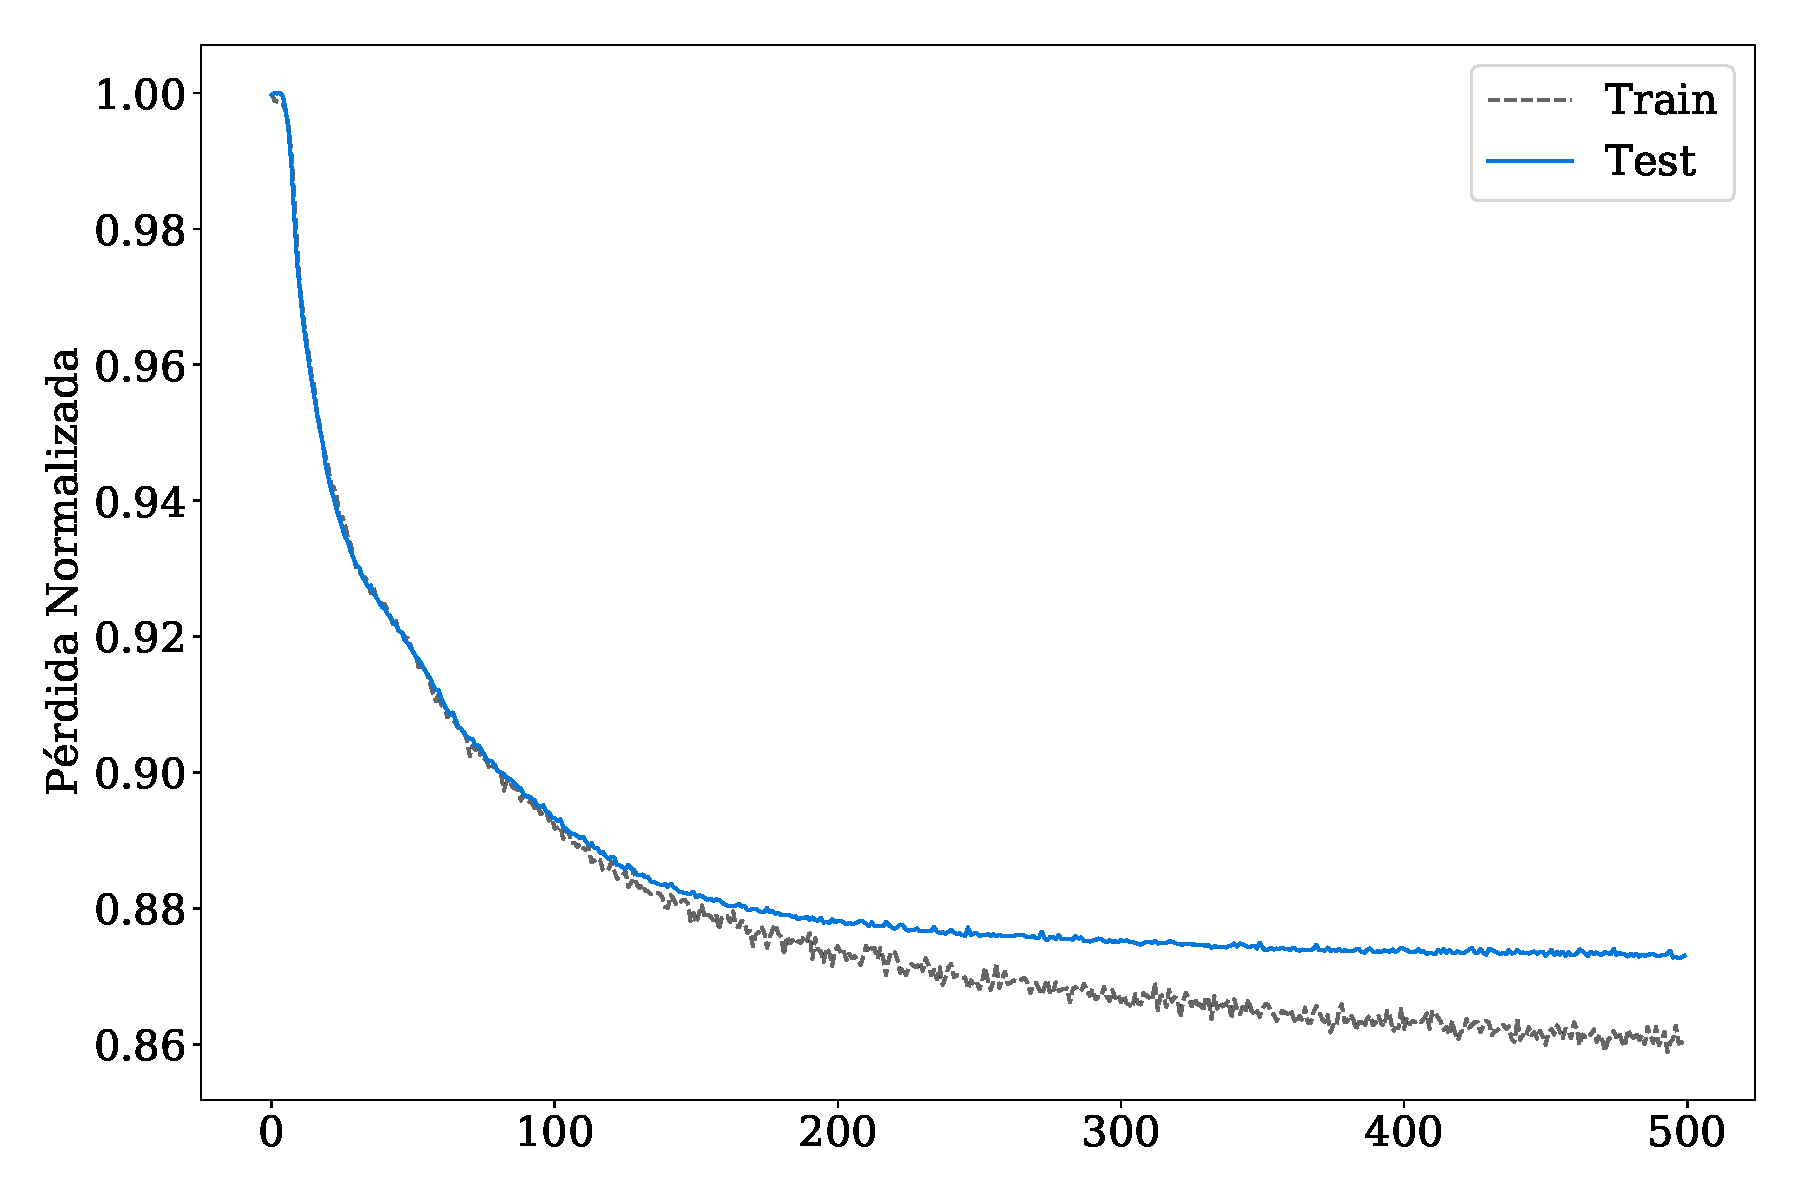
\includegraphics[width=0.5\textwidth]{Graphs/ejer3_loss.pdf}
        \end{center}
        \caption{Pérdida del entrenamiento y la  validación en función de las épocas para el  ejercicio 3.}
        \label{fig:ejer3_loss}
    \end{small}
\end{figure}

Comparando la precisión en este ejercicio, con las precisiones alcanzadas en el Soft-Max Classifier y el Support Vector Machine, como se hace en la Fig.\ref{fig:ejer3_acc_all}, la red implementada en este práctico alcanza una precisión de $40.66\%$ similar a la precisión de $40.54\%$ del Soft-Max  del ejercicio 5 de la práctica anterior. 

Considerando que usualmente al disminuir la tasa de aprendizaje, la red requiere de más épocas para converger a una solución, podemos decir que la implementación de este ejercicio tarda más en converger que los clasificadores Soft-Max y Support Vector Machine.

\begin{figure}[H]
    \begin{small}
        \begin{center}
            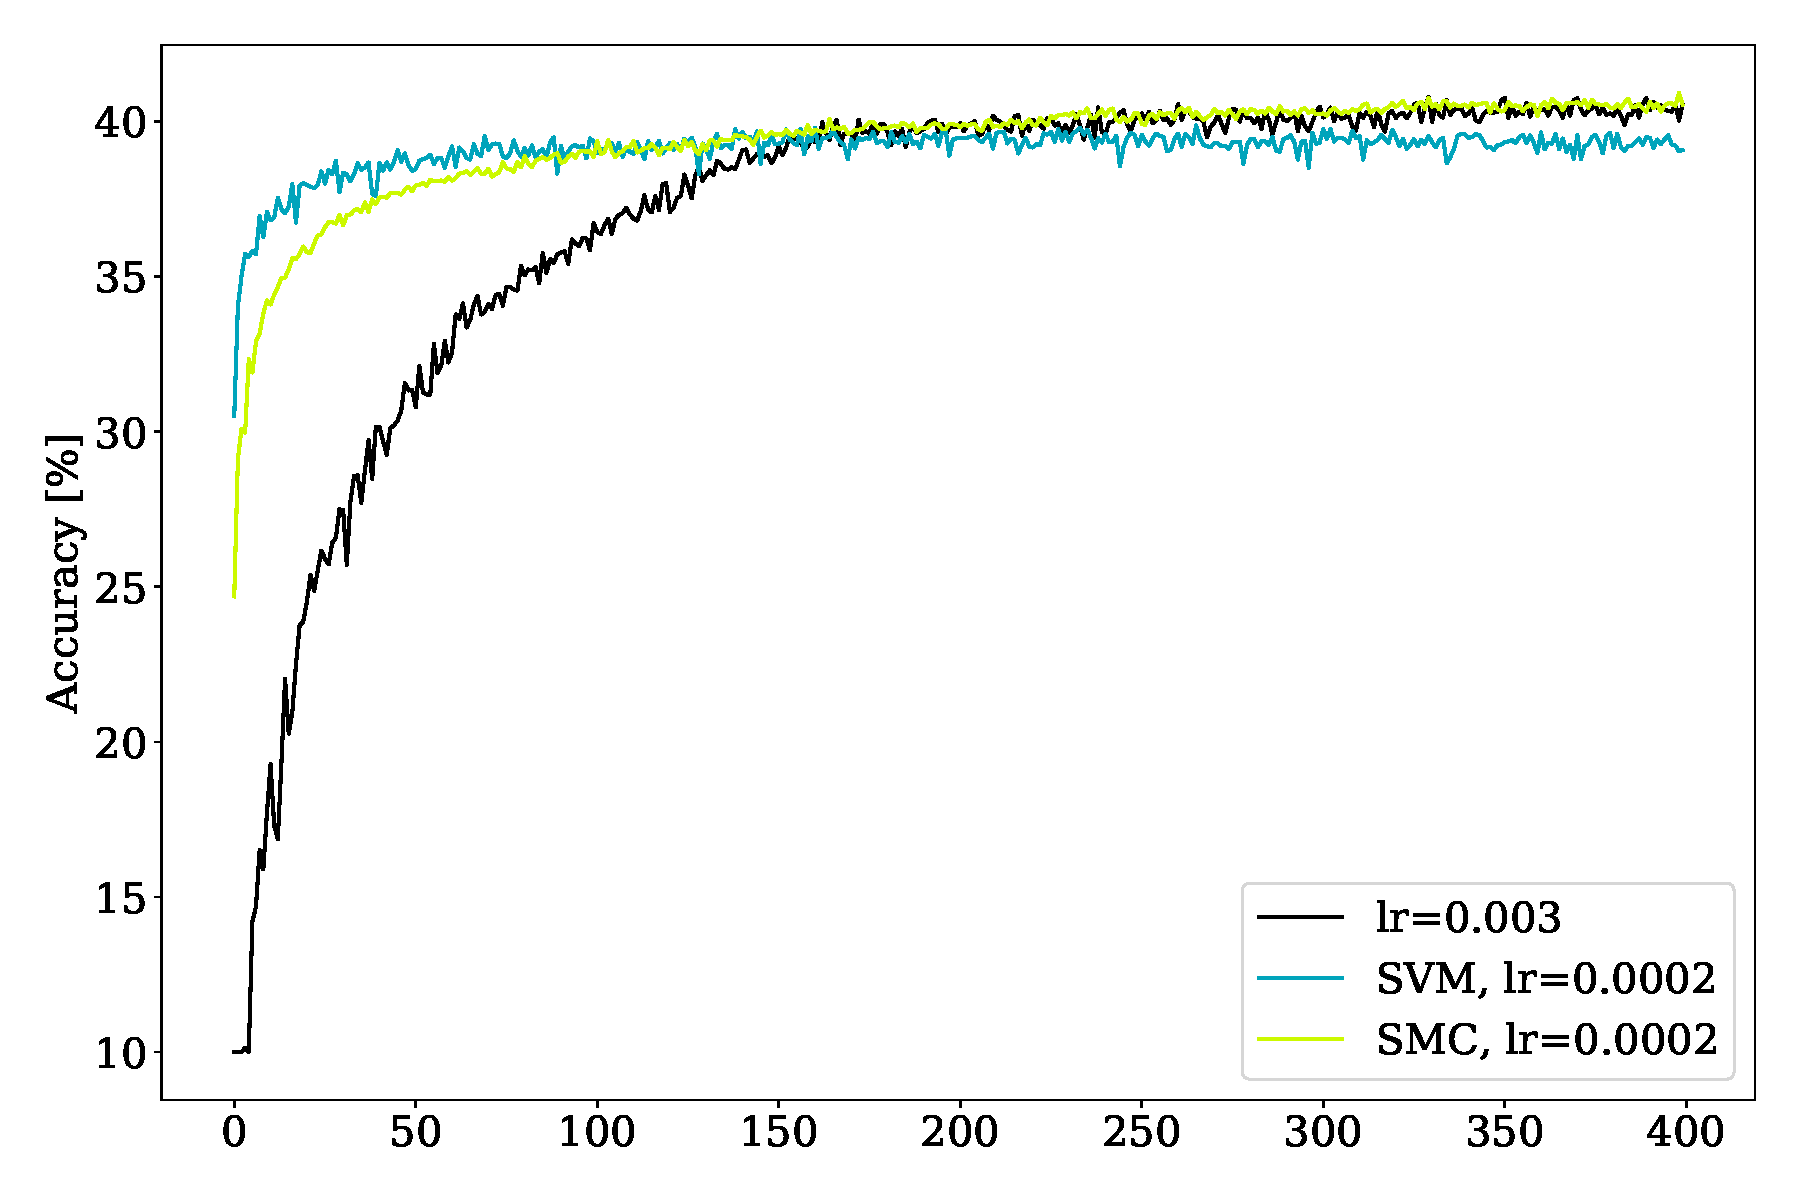
\includegraphics[width=0.5\textwidth]{Graphs/ejer3_acc_all.pdf}
        \end{center}
        \caption{Comparación de las precisiones de la conjunto de validación entre el ejercicio 3 y los clasificadores Soft-Max y Support Vector Machine de la práctica anterior.}
        \label{fig:ejer3_acc_all}
    \end{small}
\end{figure}


\subsection*{Ejercicio 4}

En este caso, las funciones de activación de la capa oculta y de salida son una función sigmoidal y lineal respectivamente, y la funciones de pérdida a comparar son la MSE y Categorical Cross-Entropy (CCE). En las Figs.\,\ref{fig:ejer4_acc} y \ref{fig:ejer4_loss} se muestran la precisión y la pérdida, normalizada por el máximo valor, función de las épocas de entrenamiento.  Se observa que la precisión alcanzada por la función de costo CCE es ligeramente superior a la precisión alcanzada por la MSE con las mismas condiciones iniciales.

\begin{figure}[H]
    \begin{small}
        \begin{center}
            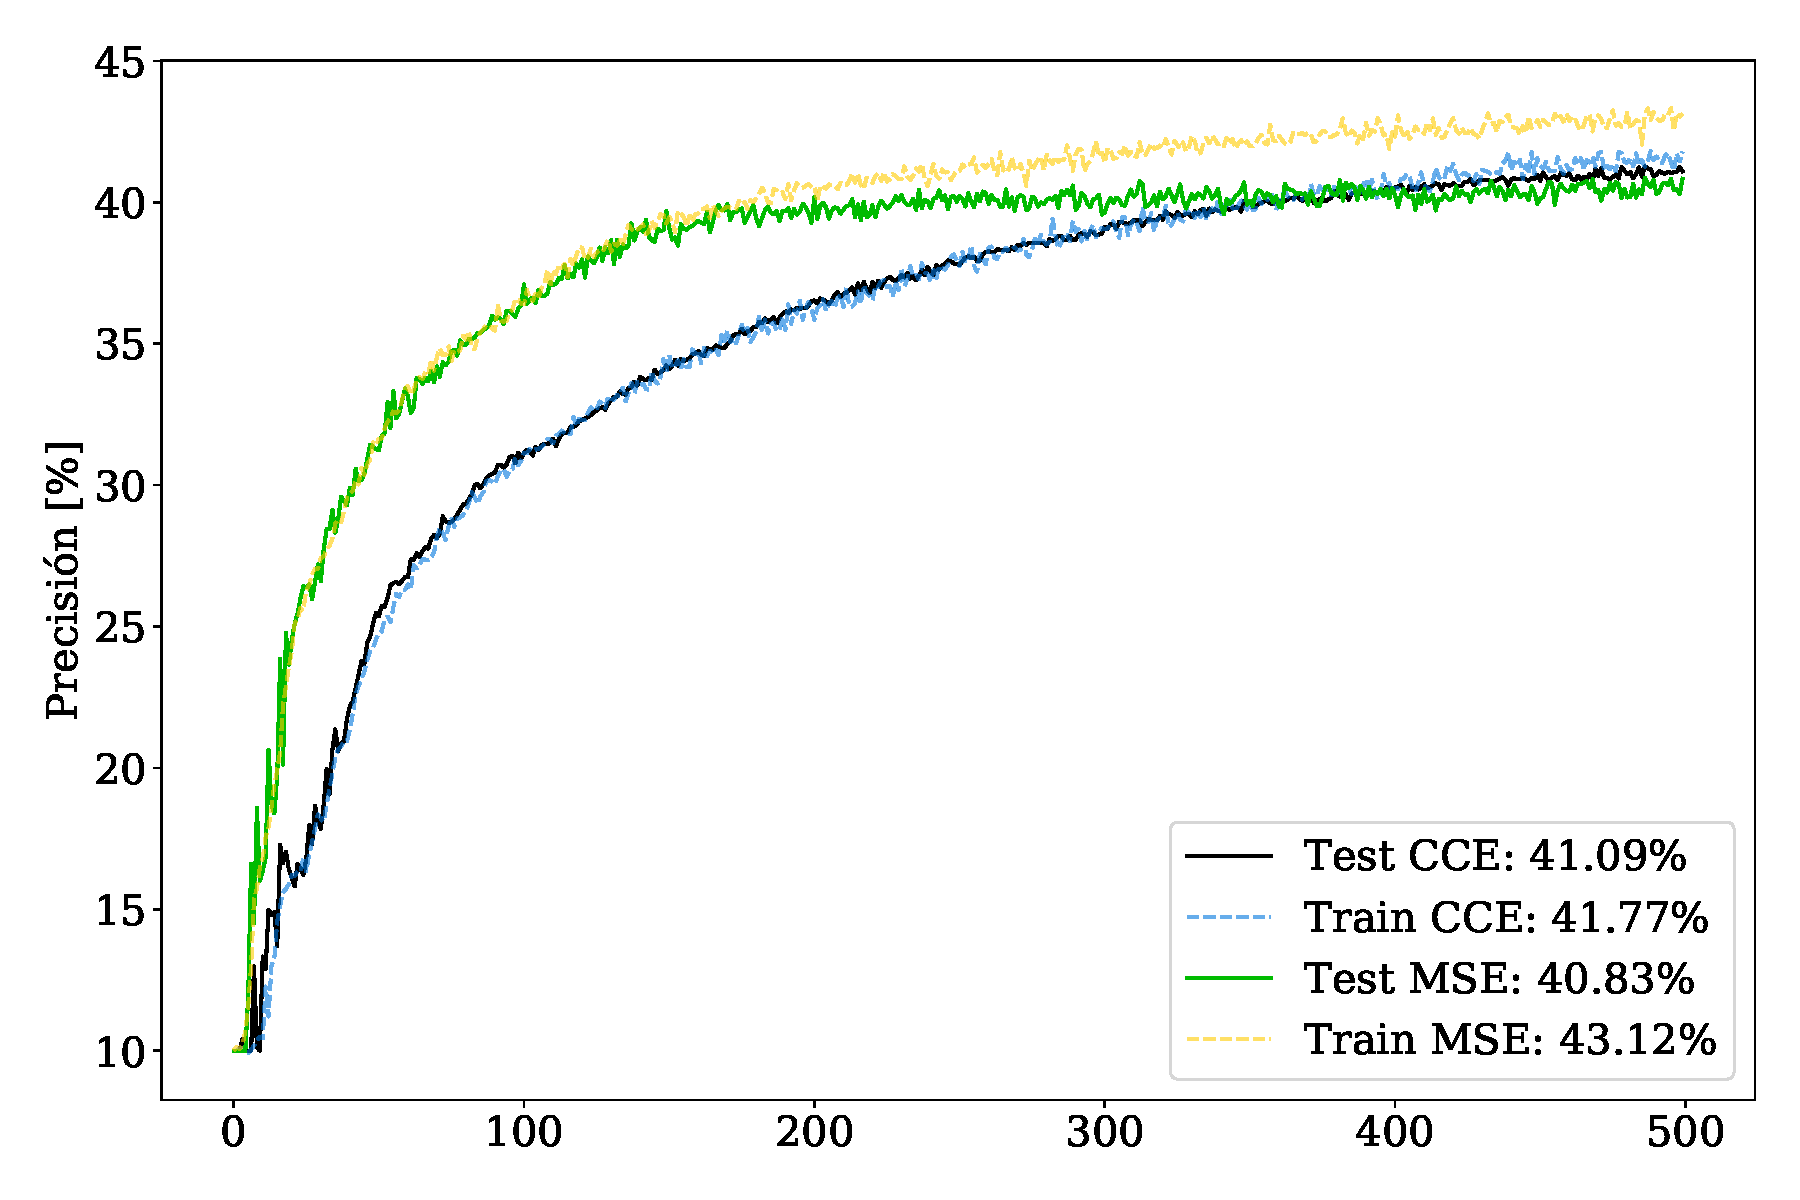
\includegraphics[width=0.5\textwidth]{Graphs/ejer4_acc.pdf}
        \end{center}
        \caption{Precisión del entrenamiento y la validación en función de las épocas para el  ejercicio 4, comparando las función de costo de MSE y CCE.}
        \label{fig:ejer4_acc}
    \end{small}
\end{figure}

\begin{figure}[H]
    \begin{small}
        \begin{center}
            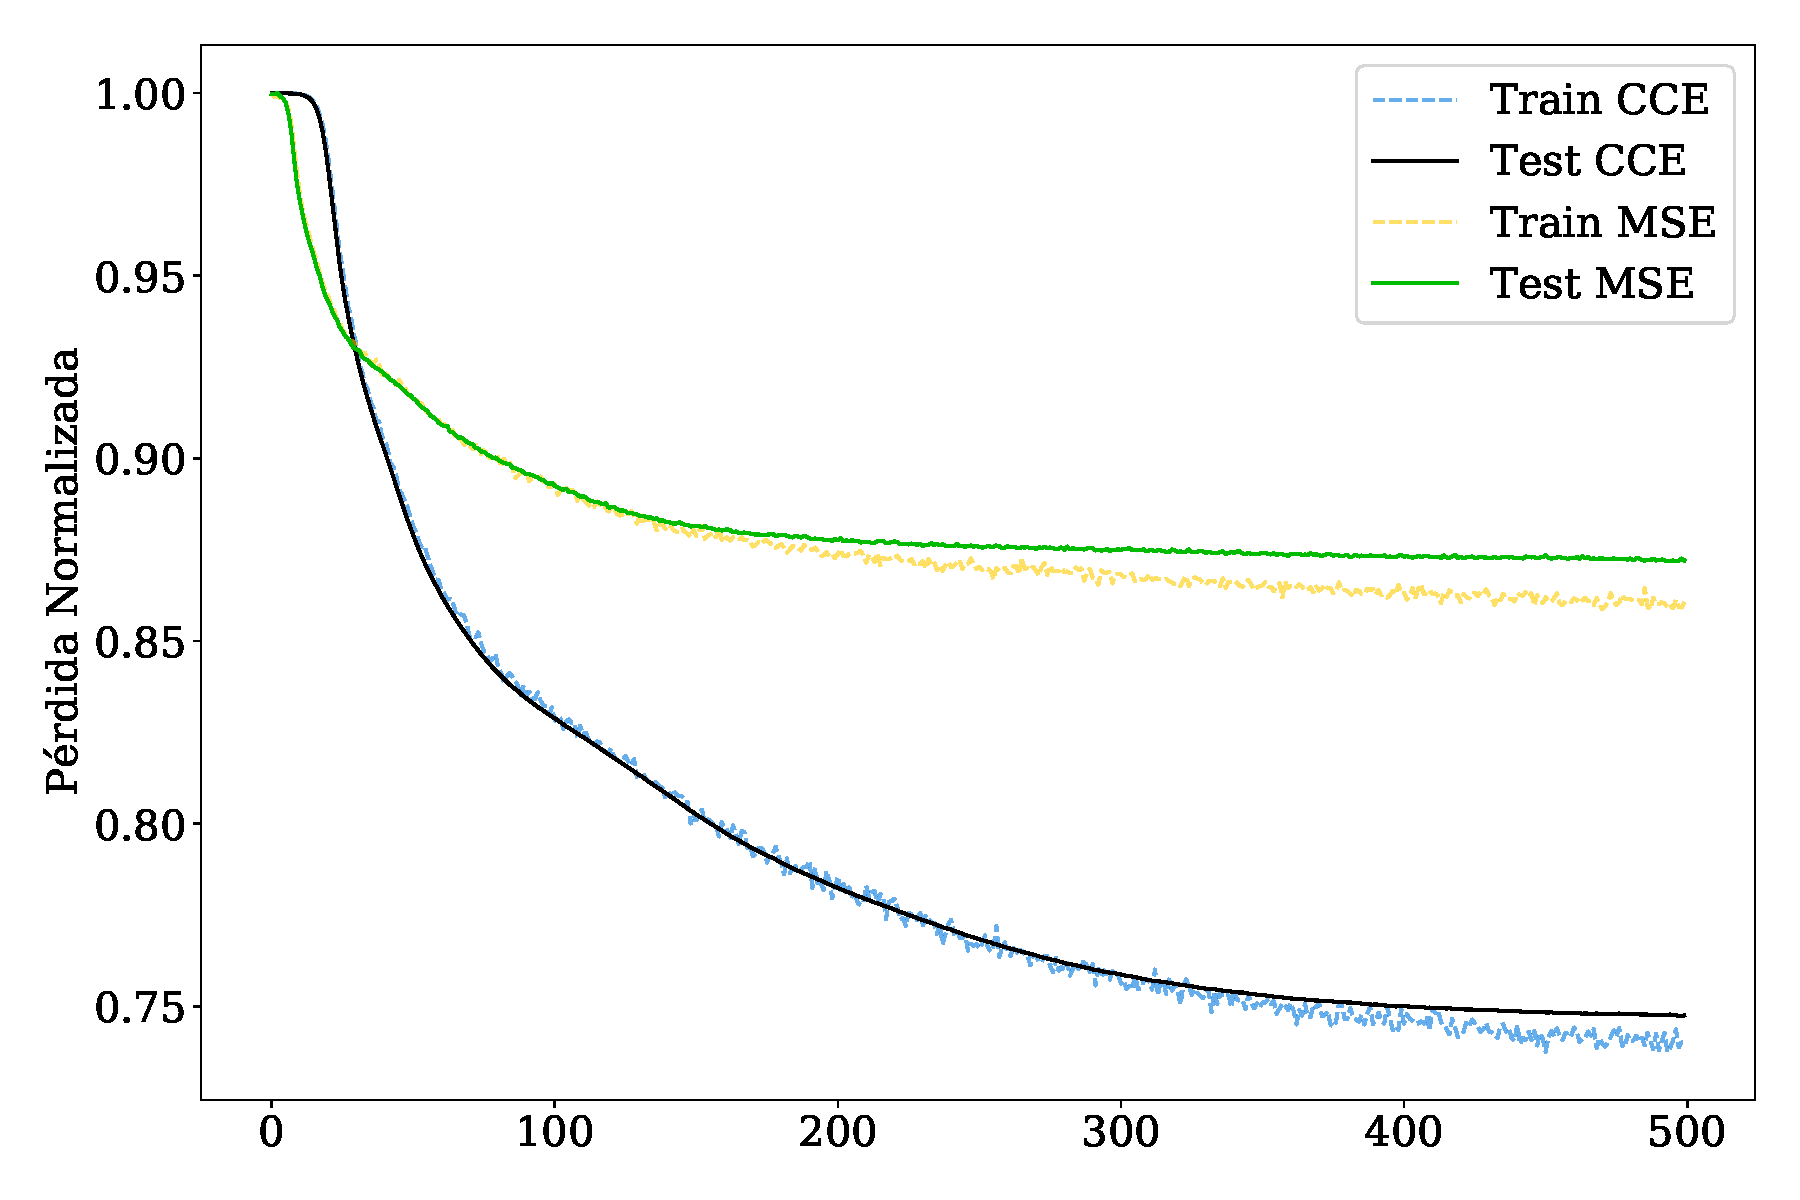
\includegraphics[width=0.5\textwidth]{Graphs/ejer4_loss.pdf}
        \end{center}
        \caption{Pérdida del entrenamiento y la  validación en función de las épocas para el  ejercicio 4, comparando las función de costo de MSE y CCE.}
        \label{fig:ejer4_loss}
    \end{small}
\end{figure}


Las valores de los parámetros de las redes son: la tasa de aprendizaje de $0.003$, y con pesos inicializados uniformemente entre $[-0.001, 0.001]$, y se utilizó un regularizador L2 con $\lambda=0.001$. Para comparar los resultados  de estas redes, se utilizaron en las ejecuciones del programa la misma semilla para los números aleatorios.

Comparando los resultados con el práctico anterior, como se muestra en la Fig.\ref{fig:ejer4_acc_all}, análogo al ejercicio 3, se necesitan más épocas para converger que con los clasificadores SMC y SVM. Cuando utilizamos la función de costo CCE, la precisión de la validación es cercana a la alcanzada por la SMC.

\begin{figure}[H]
    \begin{small}
        \begin{center}
            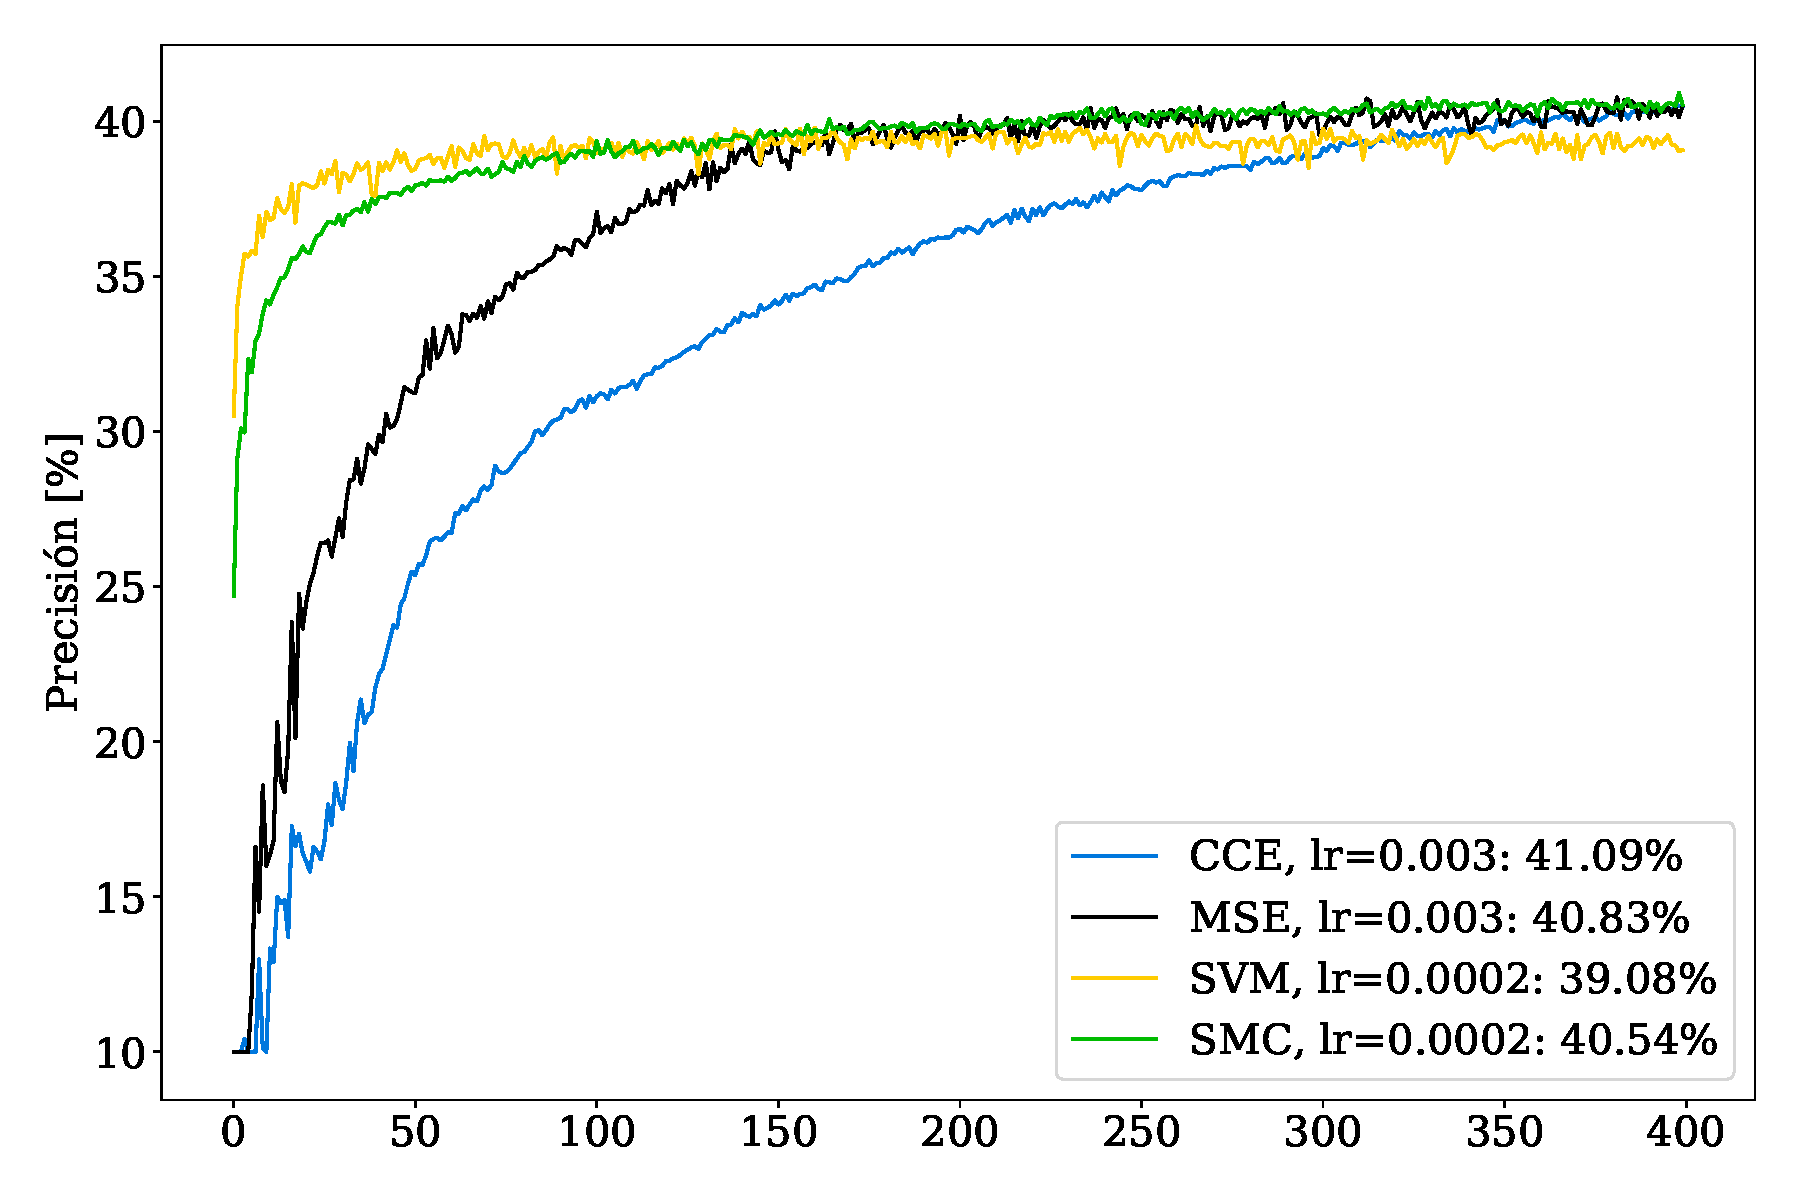
\includegraphics[width=0.5\textwidth]{Graphs/ejer4_acc_all.pdf}
        \end{center}
        \caption{Comparación de las precisiones de la conjunto de validación entre el ejercicio 4 y los clasificadores Soft-Max y Support Vector Machine de la práctica anterior.}
        \label{fig:ejer4_acc_all}
    \end{small}
\end{figure}

\begin{figure}[H]
    \begin{small}
        \begin{center}
            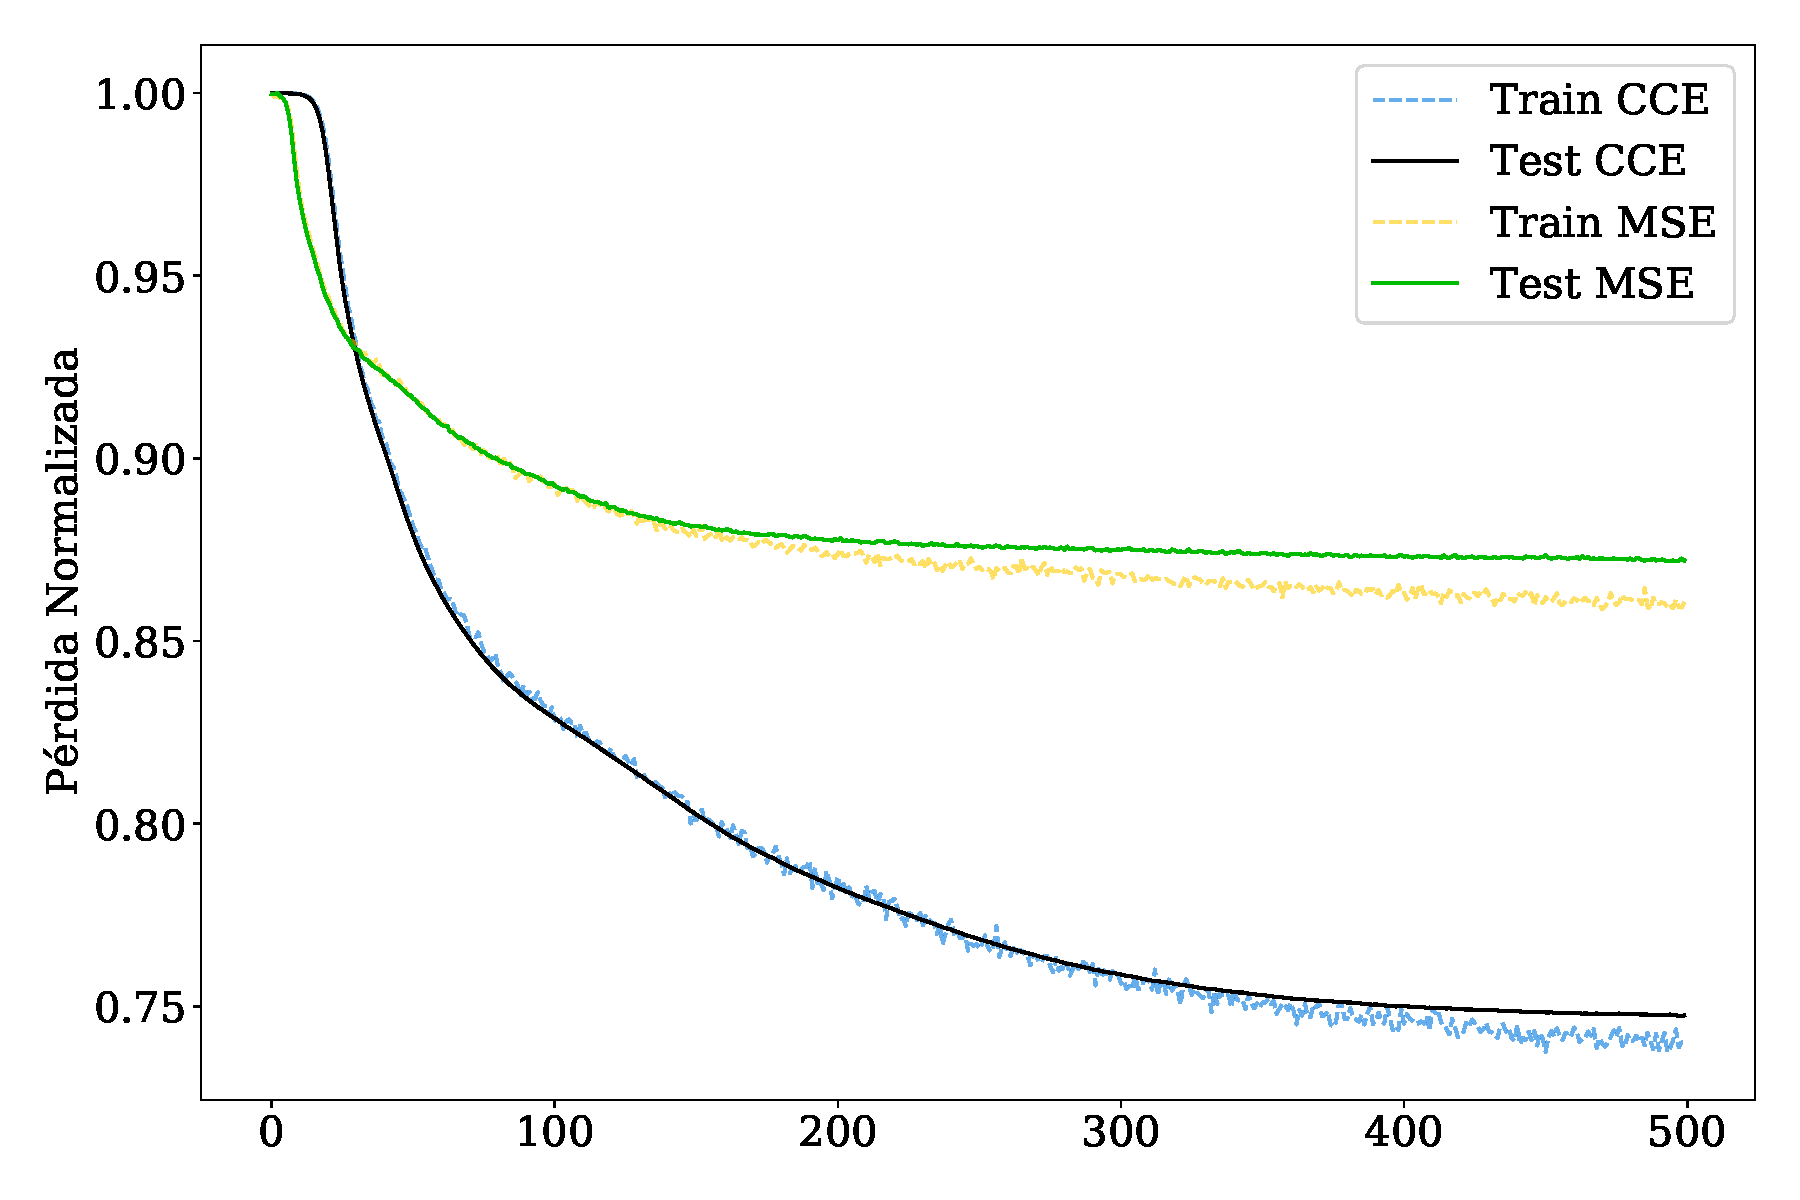
\includegraphics[width=0.5\textwidth]{Graphs/ejer4_loss.pdf}
        \end{center}
        \caption{Pérdida del entrenamiento y la  validación en función de las épocas para el  ejercicio 4, comparando las función de costo de MSE y CCE.}
        \label{fig:ejer4_loss}
    \end{small}
\end{figure}
\subsection*{Ejercicio 5}

En este caso, las funciones de activación de la capa oculta es una  función ReLU y de salida pueden ser una función sigmoidal o una función ReLU+Lineal, y la funciones de pérdida a comparar son la MSE y CCE. 

Los pesos se inicializaron de forma aleatoria entre $[-0.001, 0.001]$ para la entrada y $[-0.0001, 0.0001]$ para la capa oculta,  con una distribución uniforme. Los hiper-parámetros utilizados para las ejecuciones son $\eta$ que es la tasa de aprendizaje y $\lambda$ es el parámetro que acompaña a la función L2 en la función de regularización. Para este ejercicio, los mismos tomaron los siguientes valores:

\begin{table}[H]
    \centering
    \begin{tabular}{|l|l|l|l|l|}
    \hline
    \multicolumn{2}{|l|}{Costo}                & Activación Salida & $\eta$ & $\lambda$ \\ \hline
    \multicolumn{2}{|c|}{\multirow{2}{*}{CCE}} & Sigmoide          & 0.001  & 0.01      \\ \cline{3-5} 
    \multicolumn{2}{|c|}{}                     & ReLU+Lineal       & 0.0005 & 0.01      \\ \hline
    \multicolumn{2}{|l|}{\multirow{2}{*}{MSE}} & Sigmoide          & 0.0007 & 0.1       \\ \cline{3-5} 
    \multicolumn{2}{|l|}{}                     & ReLU+Lineal       & 0.001  & 0.01      \\ \hline
    \end{tabular}
    \caption{Tabla de hiper-parámetros del ejercicio 5.}
\end{table}


En las Figs.\,\ref{fig:ejer5_acc} y \ref{fig:ejer5_loss} se muestran la precisión y la pérdida, normalizada por el máximo valor, función de las épocas de entrenamiento.  Se observa que la precisión alcanzada por la función de costo CCE es superior a la precisión alcanzada por la MSE con ambas funciones de activación en la salida. 

Comparando las funciones de activación, la función ReLU+Lineal funciona mejor que la función sigmoidal. Considerando lo que se explicó en clase, esto se debe a que la derivada de la función sigmoidal puede ser muy pequeña cuando la función satura en 1 o en 0. En cambio la ReLU+Lineal tiene derivada no nula fuera del 0, además del cambio de derivada para números por encima y por debajo de 0.

En este ejercicio en particular, se pudo constatar la variabilidad que provoca la forma en inicializar los pesos y la funciones de activación de la capas. Se implementó otras distribuciones para los pesos pero la utilizada en este trabajo, fue la que mejor resultados brindó.

Si ahora se compara con los resultados del práctico anterior,  como se muestra en la Fig.\,\ref{fig:ejer5_acc_all}, la combinación $CCE$ con ReLU+Lineal supera ampliamente a SMC y SVM. 


\begin{figure}[H]
    \begin{small}
        \begin{center}
            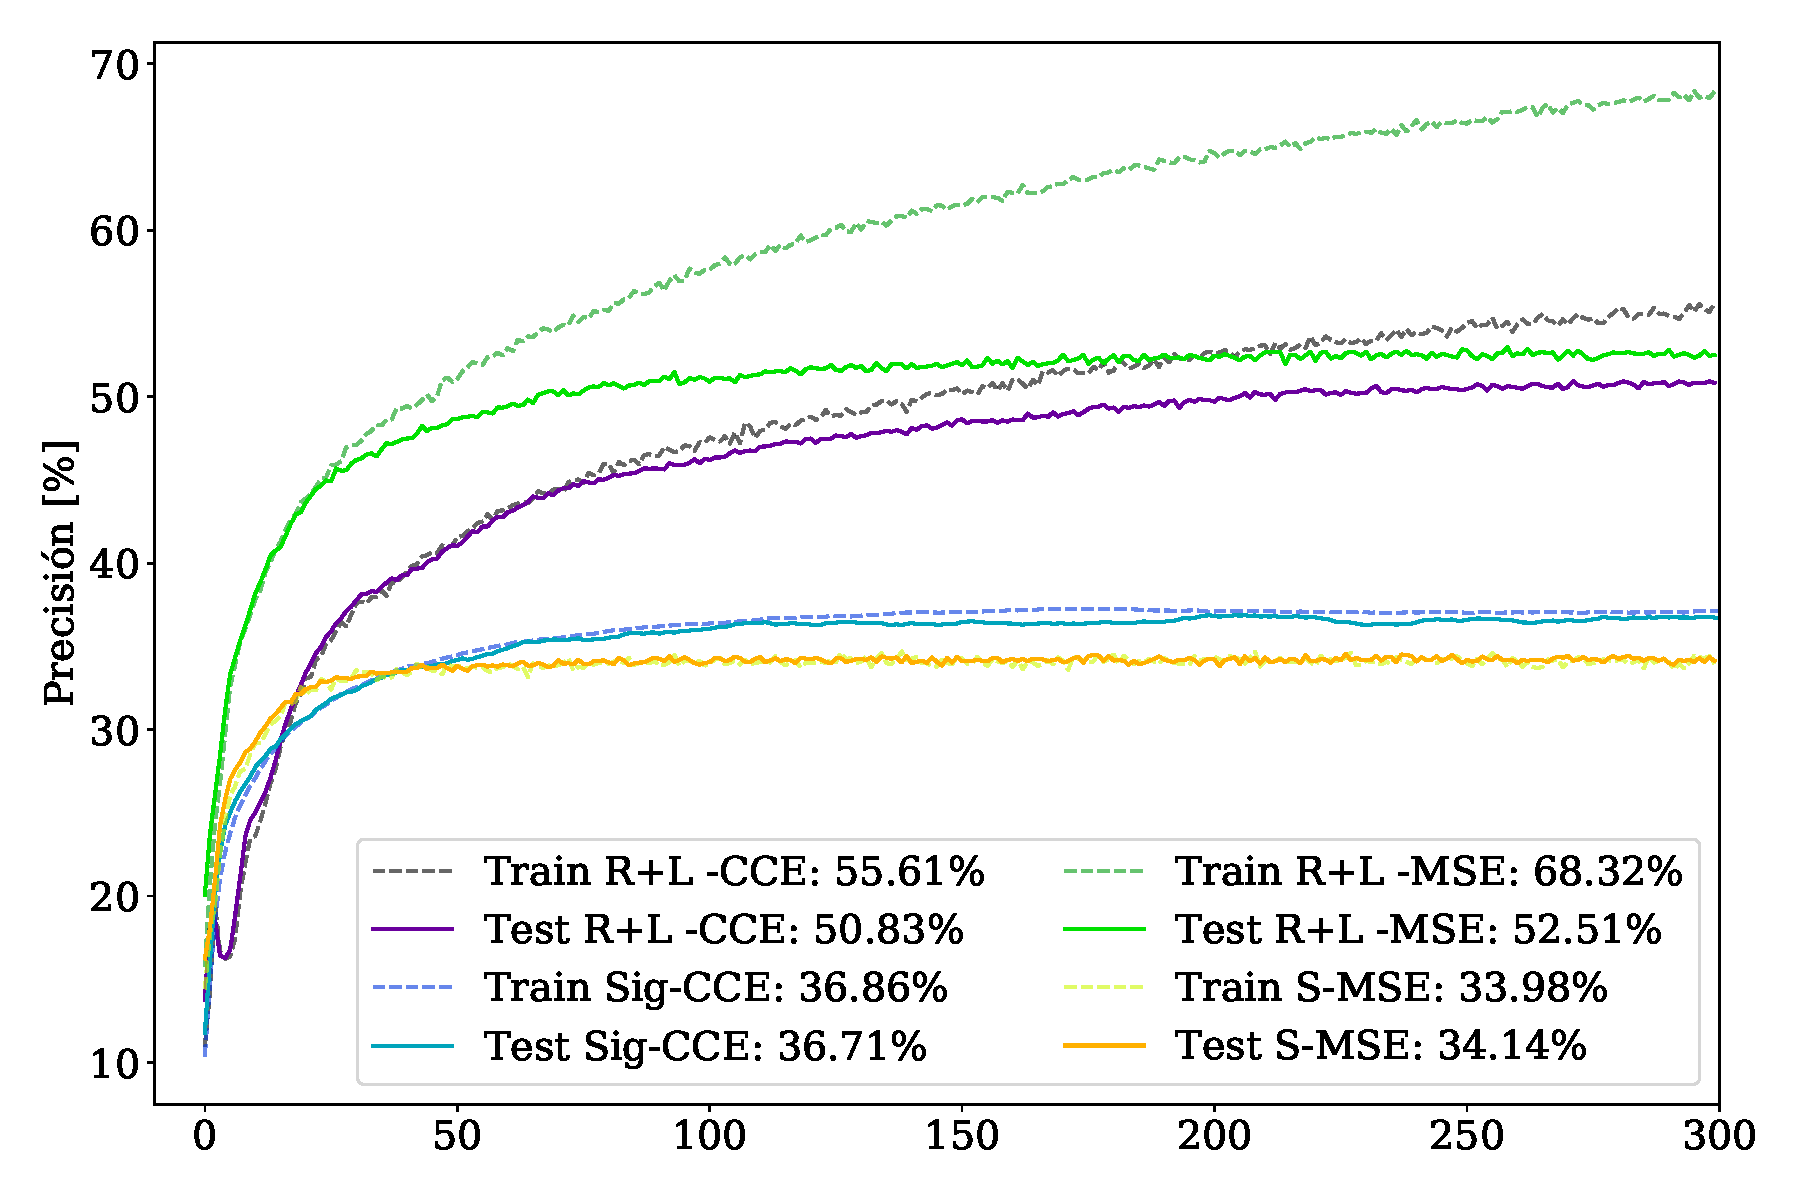
\includegraphics[width=0.5\textwidth]{Graphs/ejer5_loss.pdf}
        \end{center}
        \caption{Precisión del entrenamiento y la validación en función de las épocas para el  ejercicio 5, comparando las función de costo de MSE y CCE y las activaciones ReLU+Lineal (R+L) y Sigmoidal (S).}
        \label{fig:ejer5_acc}
    \end{small}
\end{figure}



\begin{figure}[H]
    \begin{small}
        \begin{center}
            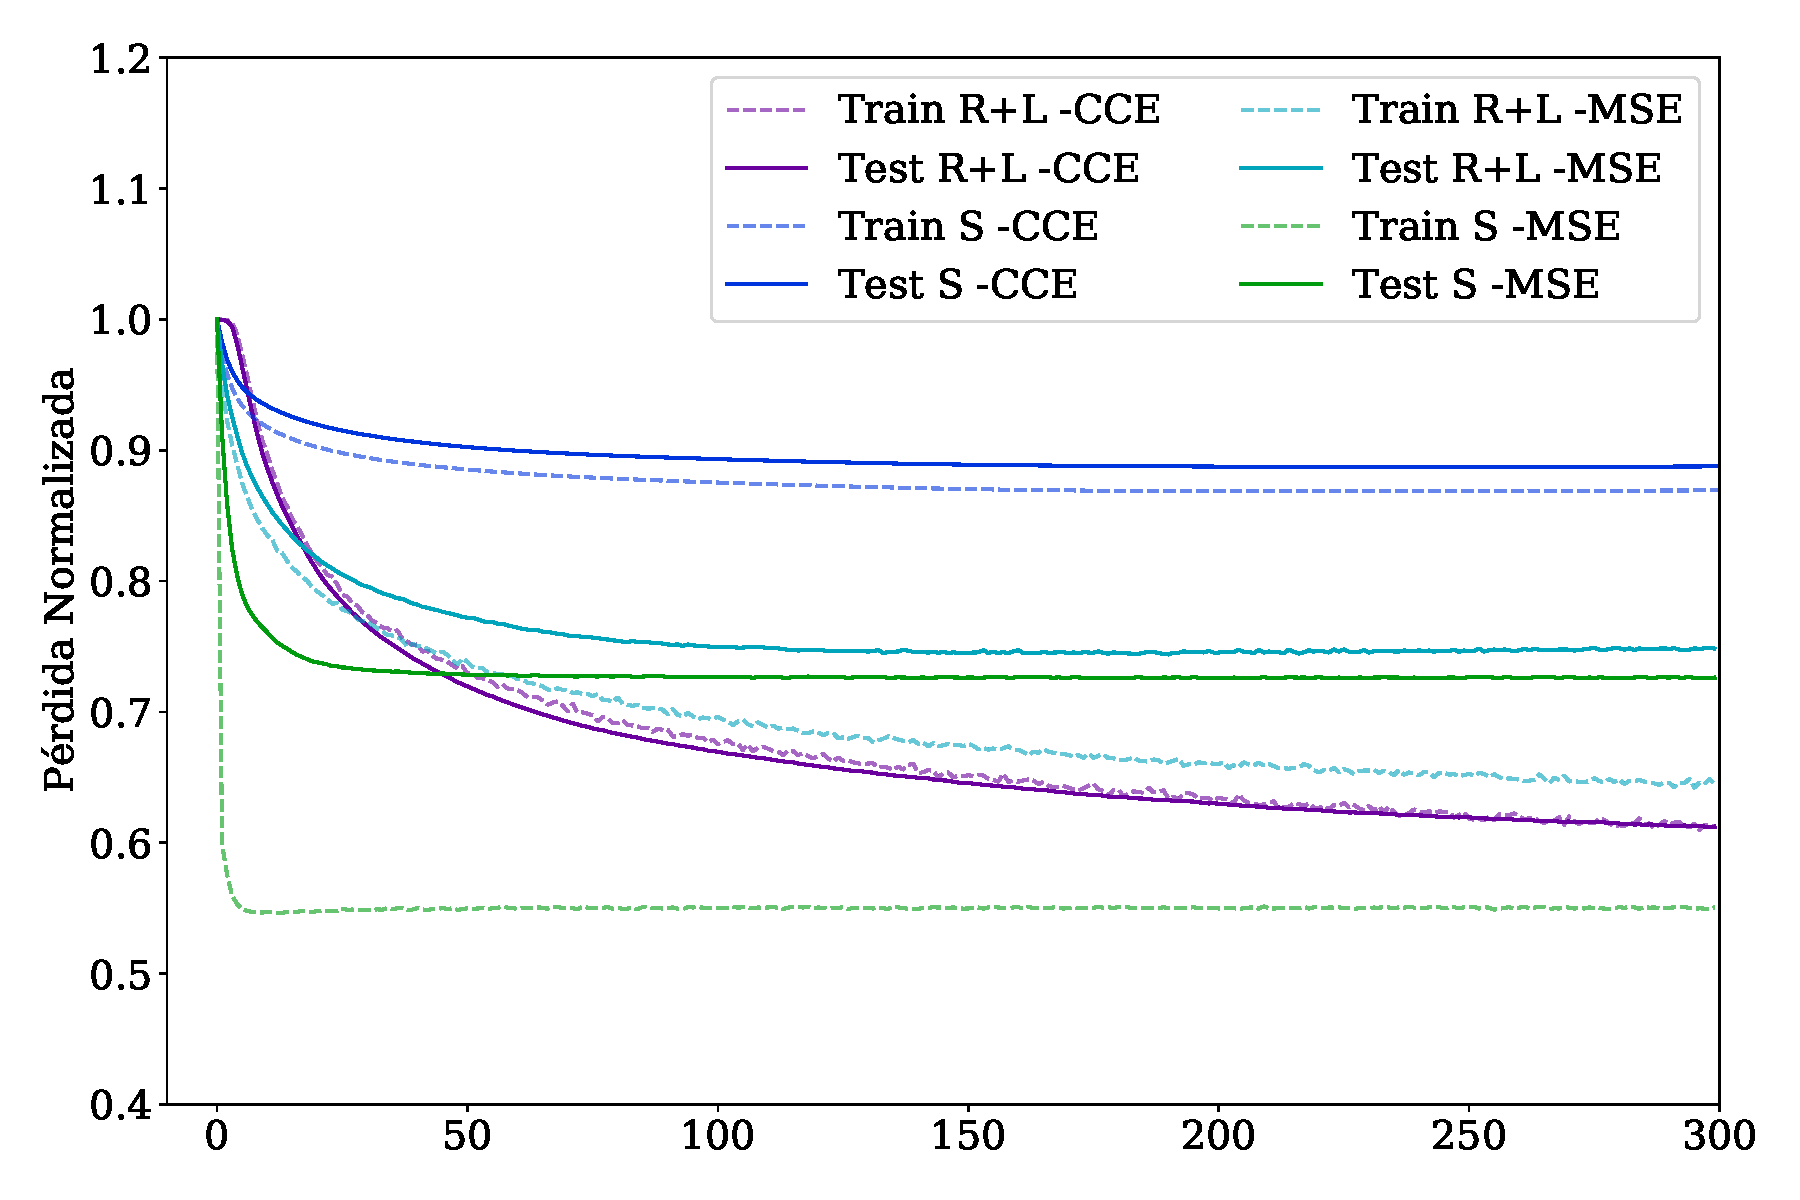
\includegraphics[width=0.5\textwidth]{Graphs/ejer5_acc.pdf}
        \end{center}
        \caption{Pérdida del entrenamiento y la validación en función de las épocas para el  ejercicio 5, comparando las función de costo de MSE y CCE y las activaciones ReLU+Lineal(R+L) y Sigmoidal (S).}
        \label{fig:ejer5_loss}
    \end{small}
\end{figure}

\begin{figure}[H]
    \begin{small}
        \begin{center}
            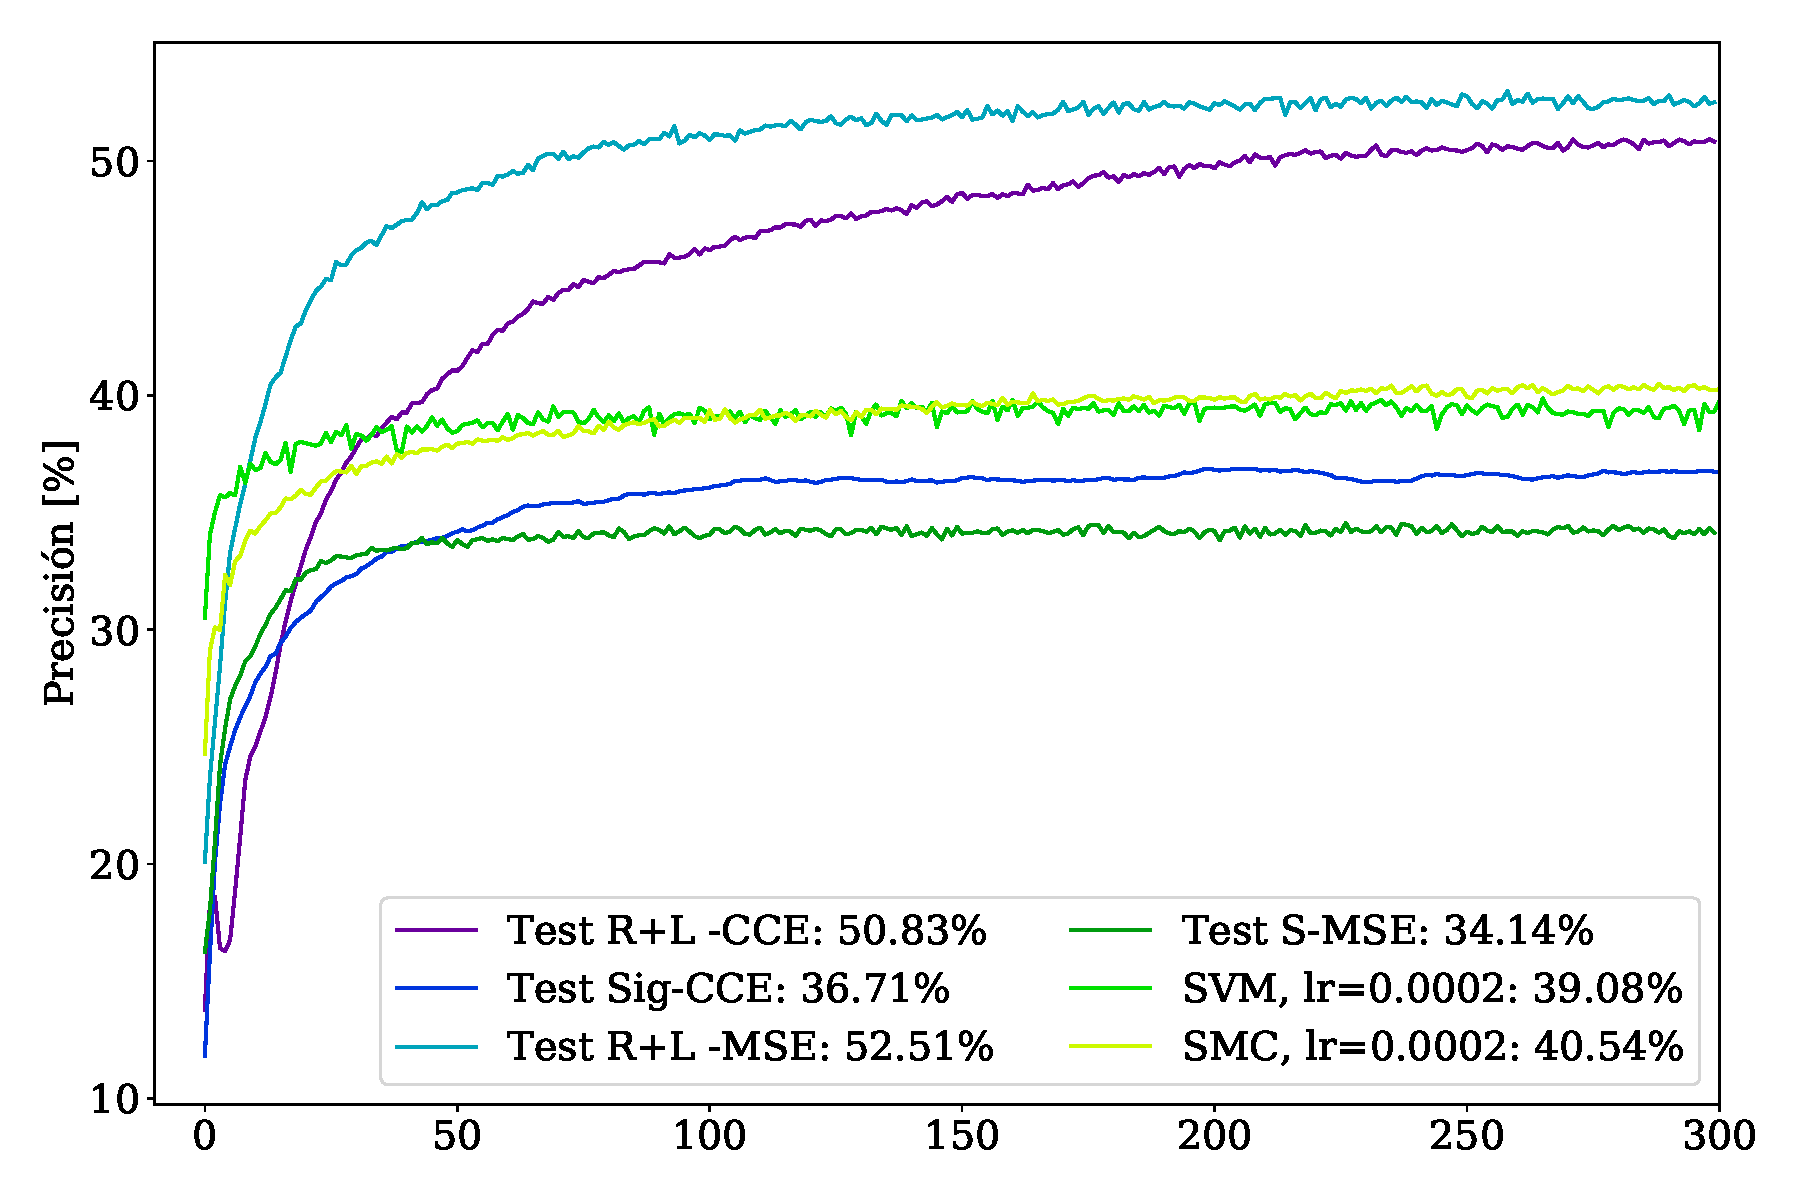
\includegraphics[width=0.5\textwidth]{Graphs/ejer5_acc_all.pdf}
        \end{center}
        \caption{Comparación de las precisiones de la conjunto de validación entre el ejercicio 5 y los clasificadores Soft-Max y Support Vector Machine de la práctica anterior.}
        \label{fig:ejer5_acc_all}
    \end{small}
\end{figure}


\section*{Resolviendo el XOR y XOR generalizado}

\subsection*{Ejercicio 6}

En este ejercicio se utilizaron dos arquitecturas para resolver el problema del XOR, las misma es completamente conectada (Fig.\,\ref{fig:221}) y la otra tiene una capa oculta con la inyección de la entrada (Fig.\,\ref{fig:211}). 

Como el XOR tiene 4 posibles casos de entrada, se utilizan todos los casos para el entrenamiento, por lo que no tenemos un conjunto de validación.  Se utilizó un tamaño de batch de 4, con una tasa de aprendizaje de $0.1$ y pesos inicializados mediante una distribución gaussiana con media nula y dispersión de $1$. 


En las Figs.\,\ref{fig:ejer6_acc} y \,\ref{fig:ejer6_loss} se muestran la precisión y la pérdida obtenidas en este ejercicio. Se observa que no hay diferencia apreciable entre ambas redes, aunque esto depende de la semilla del generador de los números aleatorios. En la ejecución de los resultados presentados se utiliza la misma semilla para ambas redes.


\begin{figure}[H]
    \centering
    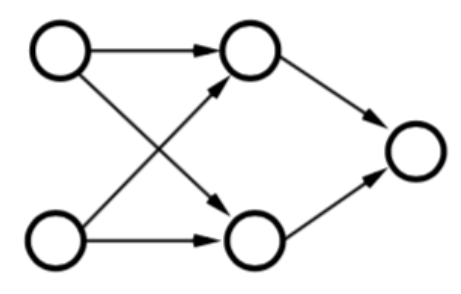
\includegraphics[width=0.27\textwidth]{Graphs/221.png}
    \caption{Arquitectura 221.}
    \label{fig:221}
\end{figure}
\begin{figure}[H]
    \centering
    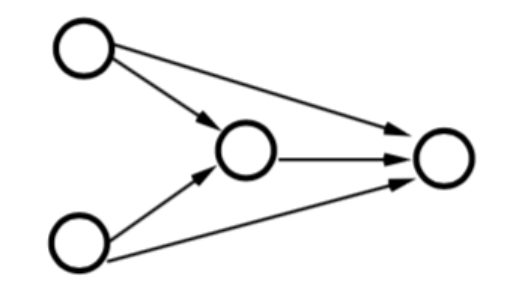
\includegraphics[width=0.27\textwidth]{Graphs/211.png}
    \caption{Arquitectura 211.}
    \label{fig:211}
\end{figure}


\begin{figure}[H]
    \centering
    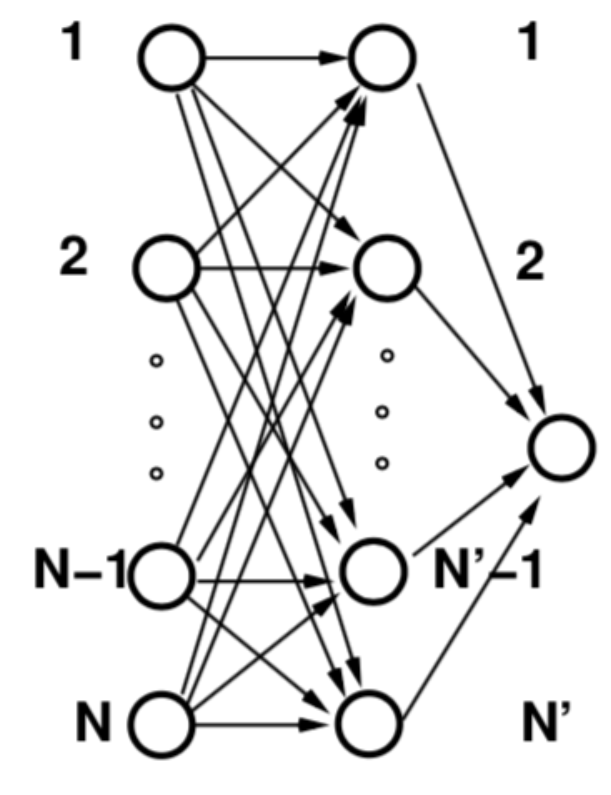
\includegraphics[width=0.27\textwidth]{Graphs/NN1.png}
    \caption{Arquitectura del problema del XOR generalizado, con un entrada $N$-dimensional, una capa oculta de $N'$.}
    \label{fig:NN1}
\end{figure}



\subsection*{Ejercicio 7}
Este ejercicio intenta resolver el XOR  generalizado, donde la función devuelve la paridad del conjunto de datos de entrada, es decir, considerando las entradas iguales a $\pm1$, si  el producto de todos los elementos de la entrada es $+1$ o $-1$.  La arquitectura del problema se esquematiza en  la Fig.\,\ref{fig:NN1}, la dimensión de la entrada se nombra como $N$ y la cantidad de neuronas en la capa oculta como $N'$.


Como el XOR generalizado tiene $2^N$ posibles casos de entrada, se utilizan todos los casos para el entrenamiento, por lo que no tenemos un conjunto de validación.  Se utilizó un tamaño de batch variable entre cada ejecución. Usamos la nomenclatura $(N,N',Ejemplos)$ para expresar la dimensión, la cantidad de neuronas en la capa oculta y el tamaño de batch. Se entrenó con una tasa de aprendizaje de $0.1$ y pesos inicializados mediante una distribución gaussiana con media nula y dispersión de $1$. También se experimentó con la cantidad de neuronas en la capa oculta $N'$.


\begin{figure}[H]
    \begin{small}
        \begin{center}
            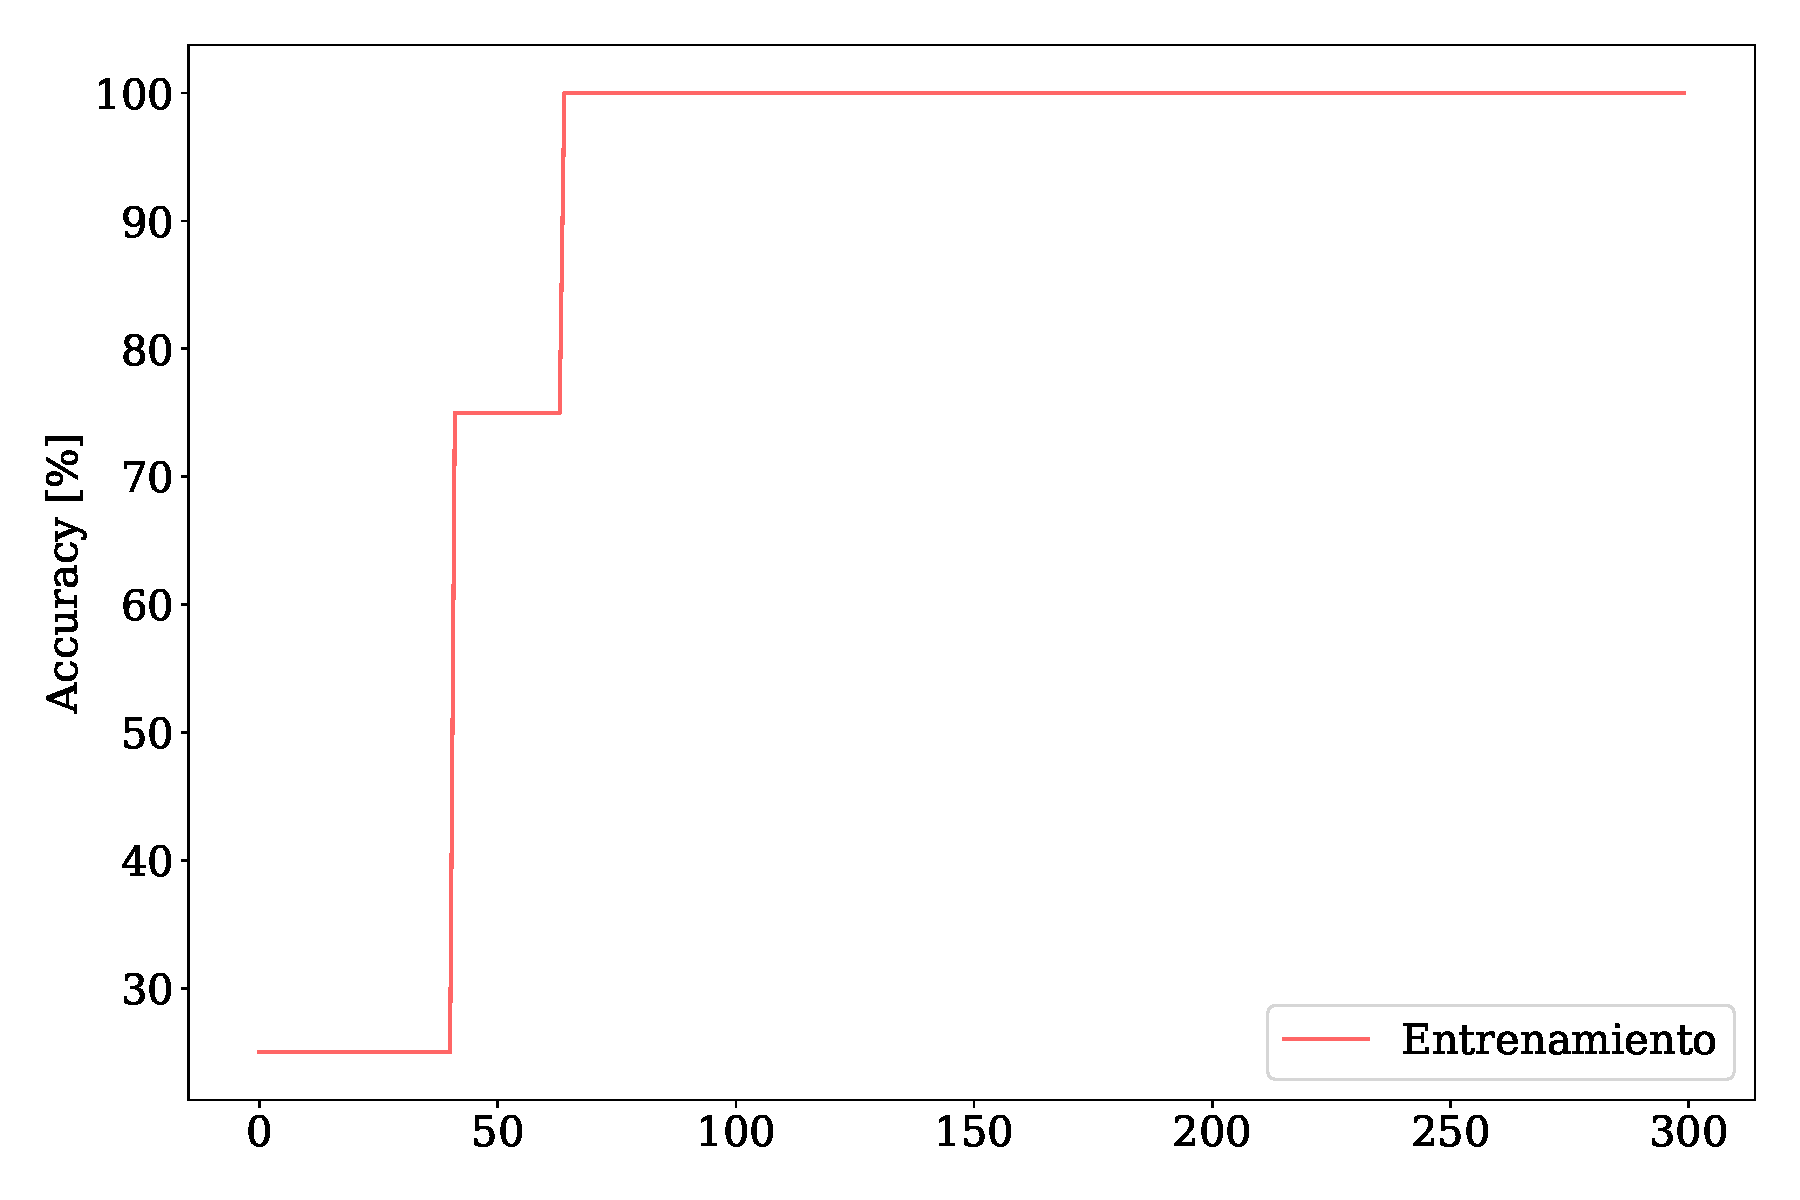
\includegraphics[width=0.5\textwidth]{Graphs/ejer6_acc.pdf}
        \end{center}
        \caption{Precisión del entrenamiento  y validación en función de las épocas para las dos redes implementadas en el ejercicio 6.}
        \label{fig:ejer6_acc}
    \end{small}
\end{figure}


\begin{figure}[H]
    \begin{small}
        \begin{center}
            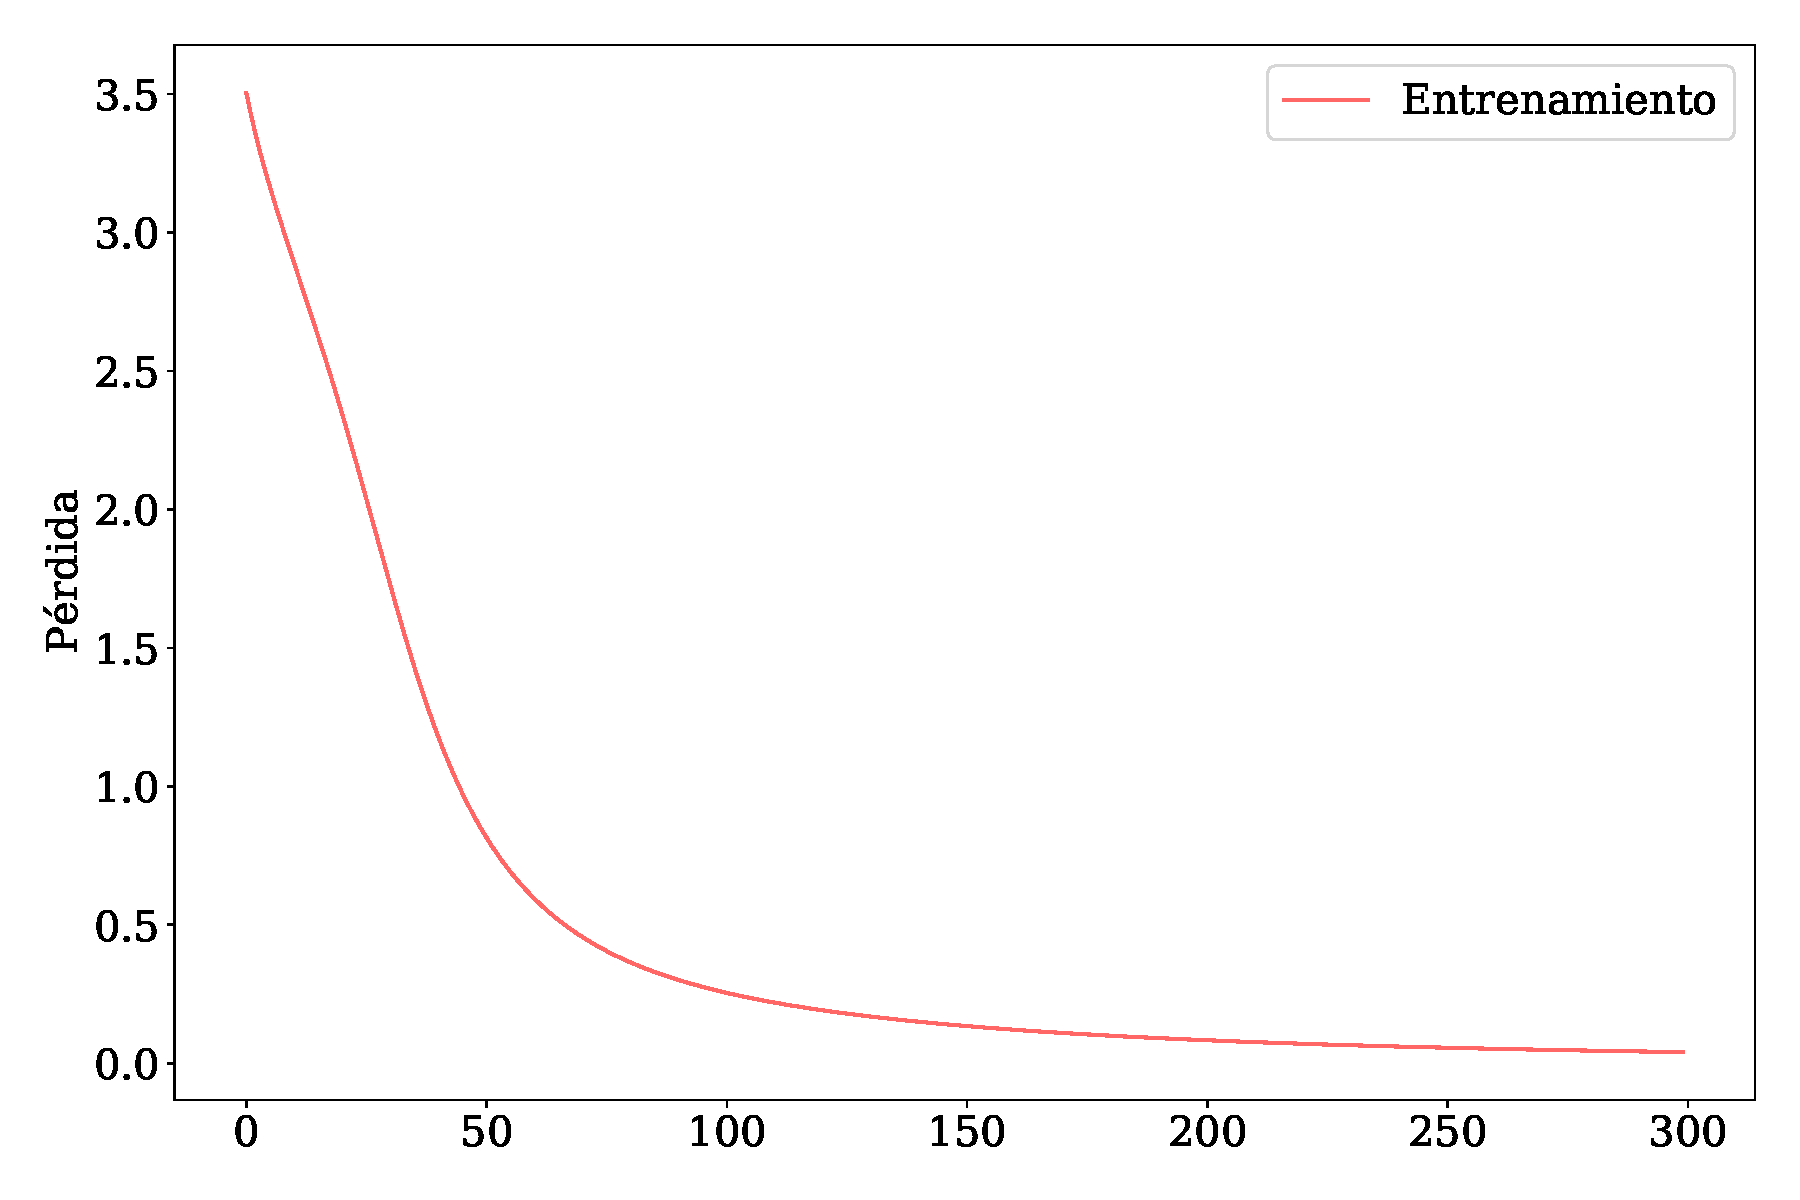
\includegraphics[width=0.5\textwidth]{Graphs/ejer6_loss.pdf}
        \end{center}
        \caption{Pérdida normalizada del entrenamiento  y validación en función de las épocas para las dos redes implementadas en el ejercicio 6.}
        \label{fig:ejer6_loss}
    \end{small}
\end{figure}


En las Figs.\,\ref{fig:ejer7_acc} y \ref{fig:ejer7_loss} se muestran las precisiones y pérdida para distintos valor de $N$ y $N'$.  En el caso de $N'\geq N$, la red se desempeña mejor, es decir alcanza una mejor precisión,  que cuando $N'<N$.

\begin{figure}[H]
    \begin{small}
        \begin{center}
            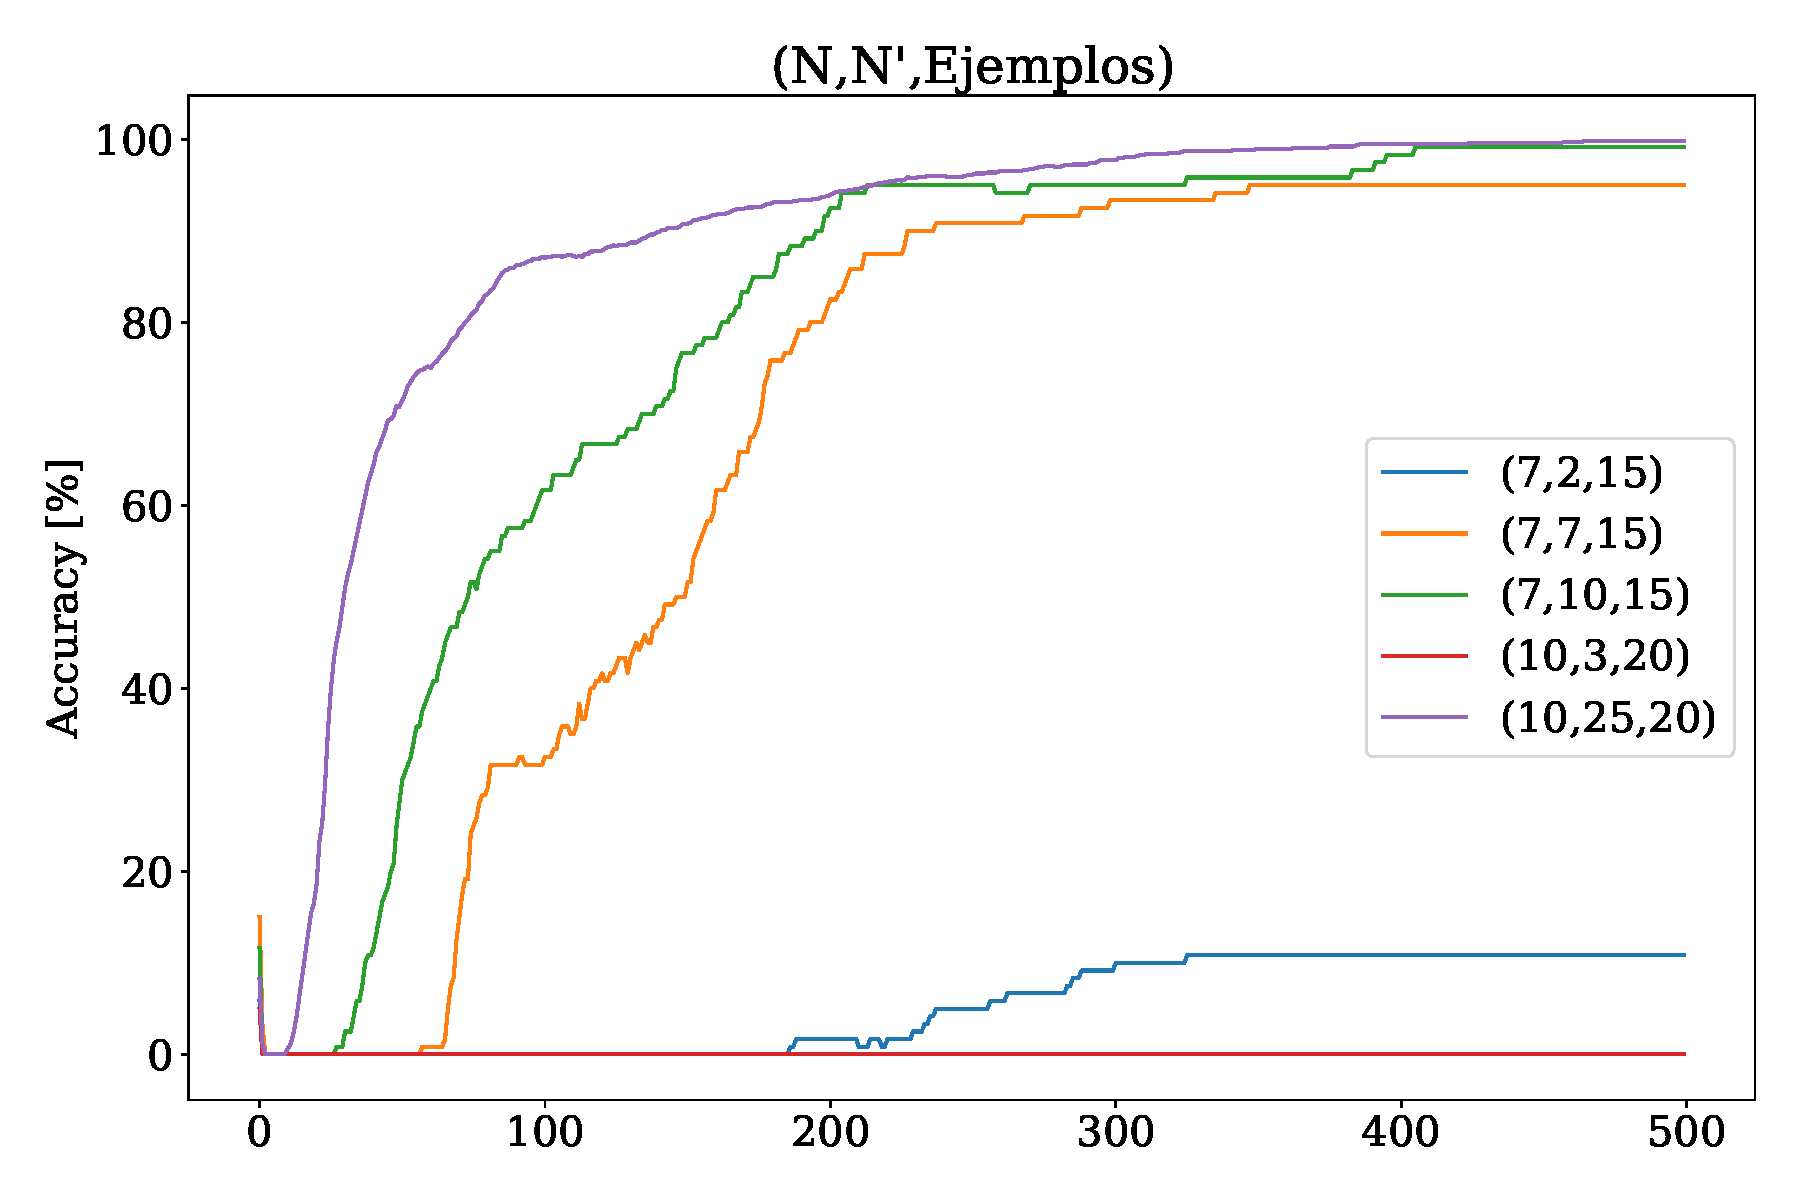
\includegraphics[width=0.465\textwidth]{Graphs/ejer7_acc.pdf}
        \end{center}
        \caption{Precisión para el XOR generalizado para distintas dimensiones ($N$), neuronas $N'$ y tamaño de batch ($Ejemplos$).}
        \label{fig:ejer7_acc}
    \end{small}
\end{figure}


\begin{figure}[H]
    \begin{small}
        \begin{center}
            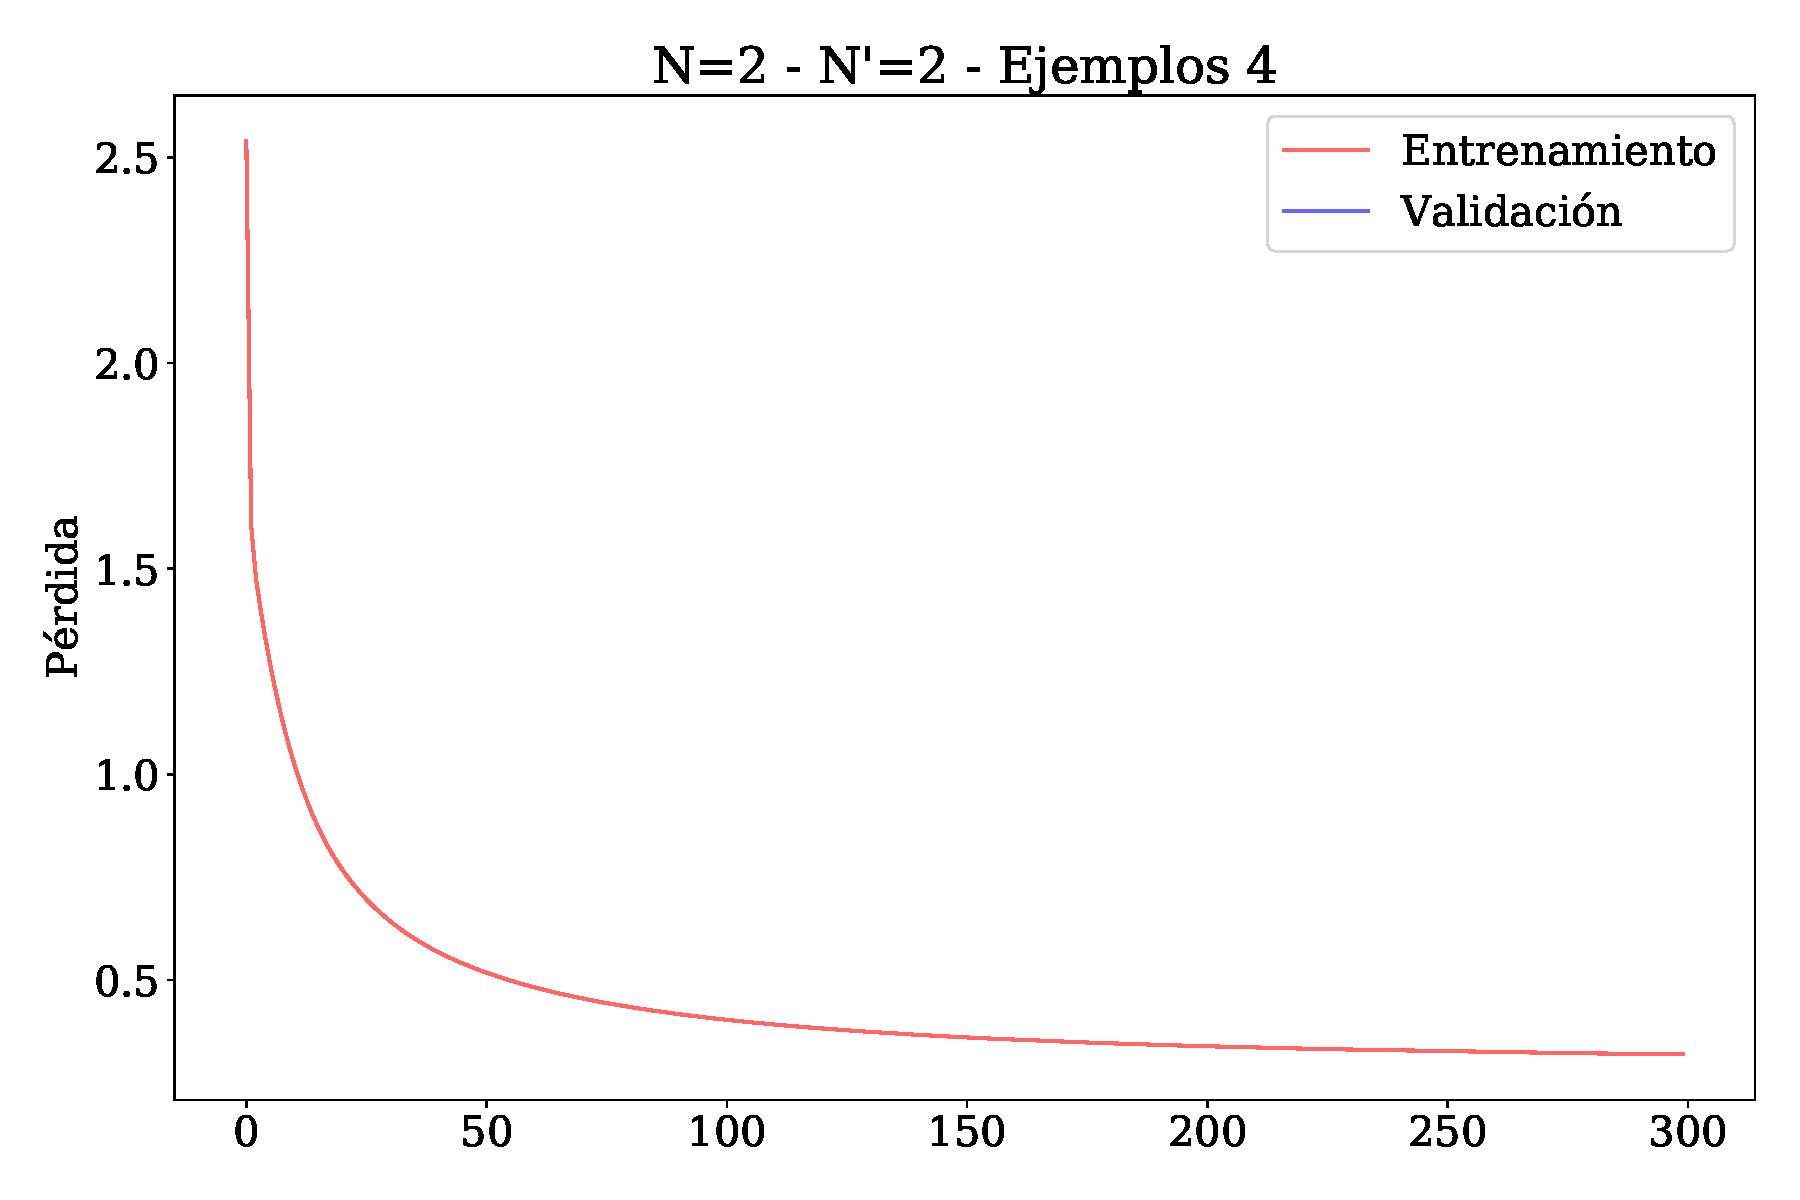
\includegraphics[width=0.465\textwidth]{Graphs/ejer7_loss.pdf}
        \end{center}
        \caption{Pérdida normalizada para el XOR generalizado para distintas dimensiones ($N$), neuronas $N'$ y tamaño de batch ($Ejemplos$).}
        \label{fig:ejer7_loss}
    \end{small}
\end{figure}

\section*{Clasificando el CIFAR-10 con dos capas ocultas}

\subsection*{Ejercicio 8}
Para el ejercicio 8, se utiliza un arquitectura de entrada, una capa oculta de 100 neuronas, una segunda capa oculta de 100 neuronas con la misma función de activación que la anterior, y una capa oculta con activación lineal. 

En este trabajo se probaron las funciones ReLU y sigmoidal en las dos capas, con la función de costo MSE.  Con los pesos inicializados con una distribución gaussiana de media nula y dispersión 0.07. Los hiper-parámetros $\eta$ y $\lambda$ tomaron los valores $0.001$ y $0.1$ respectivamente, con una función L2 para la regularización. Se observó que con este valor de  $\lambda$ se evita el overfitting de la red.

En las Figs.\,\ref{fig:ejer8_acc}  y \ref{fig:ejer8_loss} se muestran la precisión y la pérdida respectivamente, se observa que la precisión en los datos de validación,   con la función de activación ReLU, llega a un valor de $46.33\%$. En este ejercicio nuevamente, el ReLU supera en precisión a la sigmoidal.


\begin{figure}[H]
    \begin{small}
        \begin{center}
            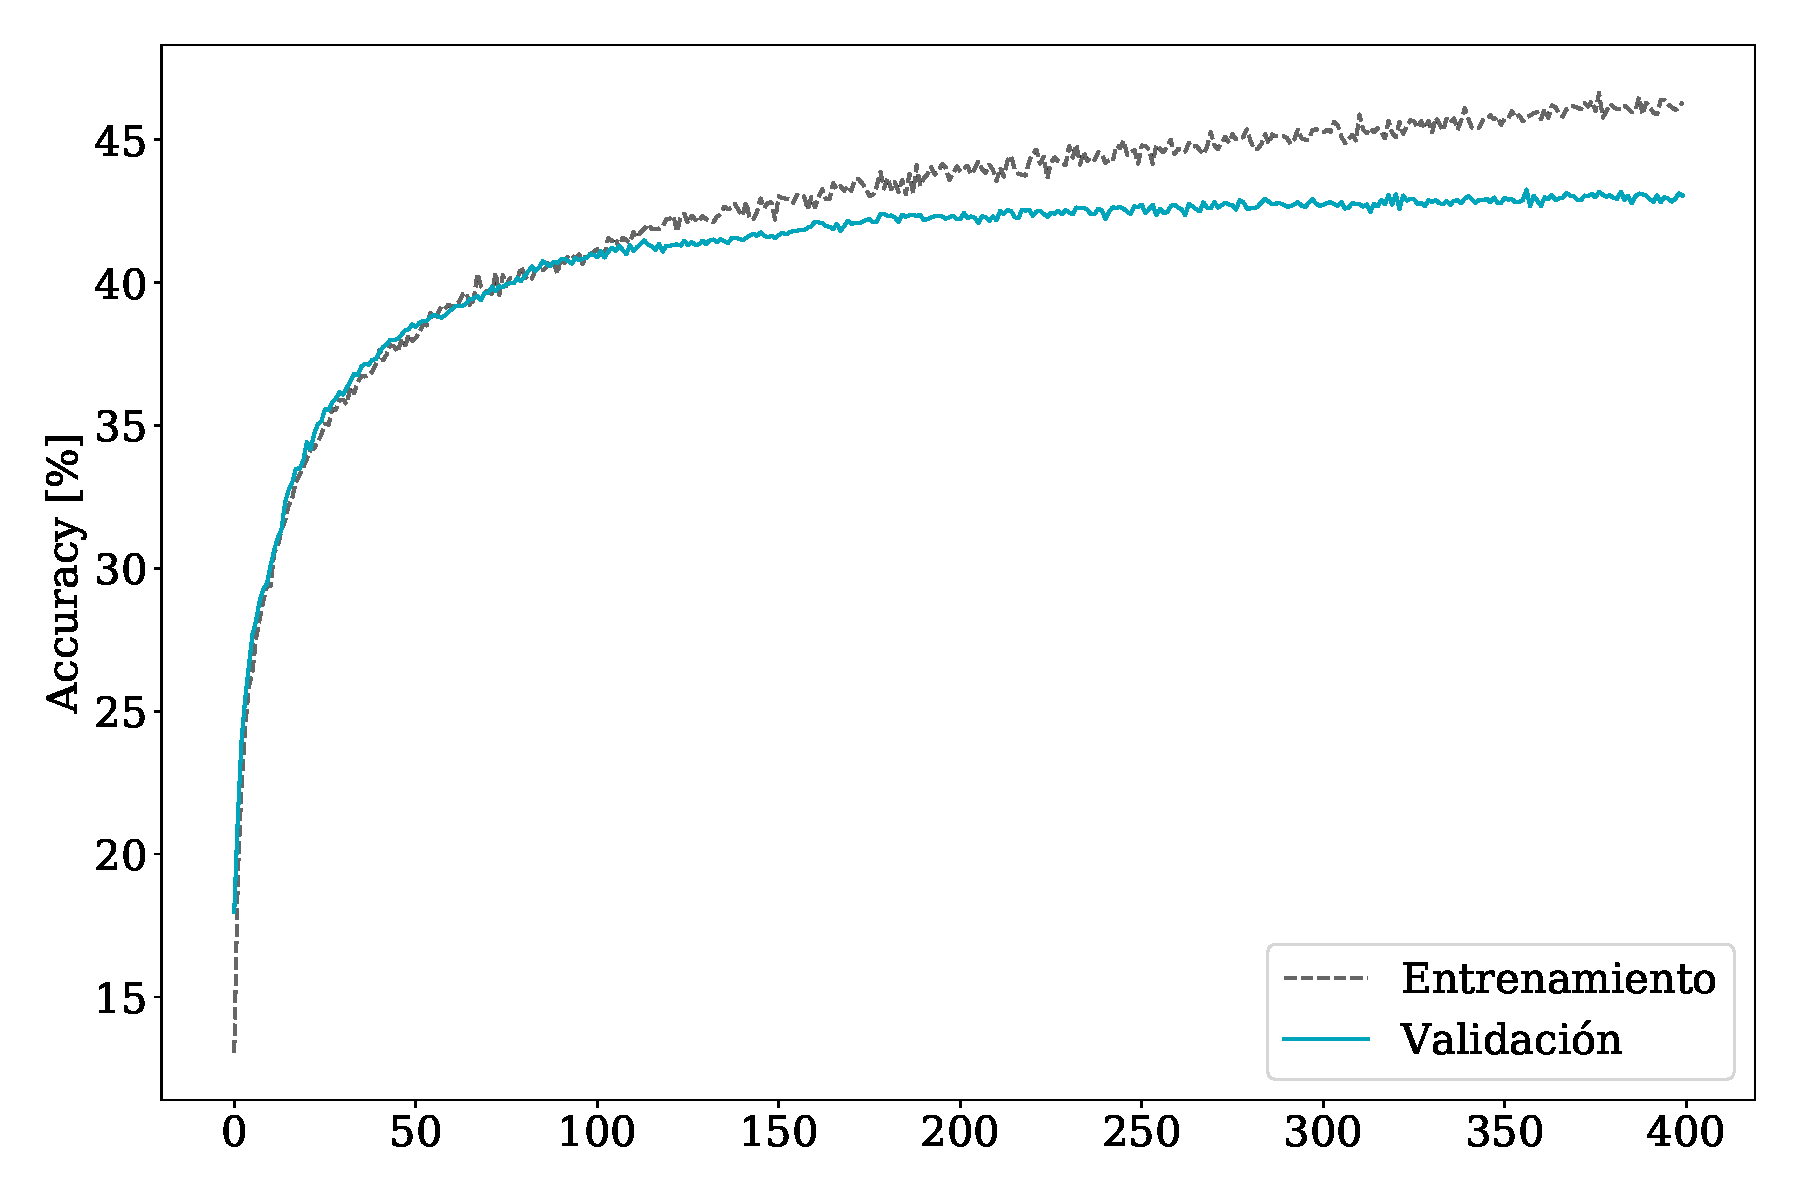
\includegraphics[width=0.465\textwidth]{Graphs/ejer8_acc.pdf}
        \end{center}
        \caption{Precisión del entrenamiento y validación en función de las épocas para las dos redes implementadas en el ejercicio 8.}
        \label{fig:ejer8_acc}
    \end{small}
\end{figure}

En la Fig.\,\ref{fig:ejer8_acc_all} se observa que clasificadores  SMC y SVM, y el ejercicio 3, obtienen una mejor precisión que al usar la función sigmoidal como activación en esta arquitectura. Cuando se utiliza en cambio la función ReLU, los resultados son mejores, comprobando la ventaja de la ReLU sobre la función sigmoidal.

\begin{figure}[H]
    \begin{small}
        \begin{center}
            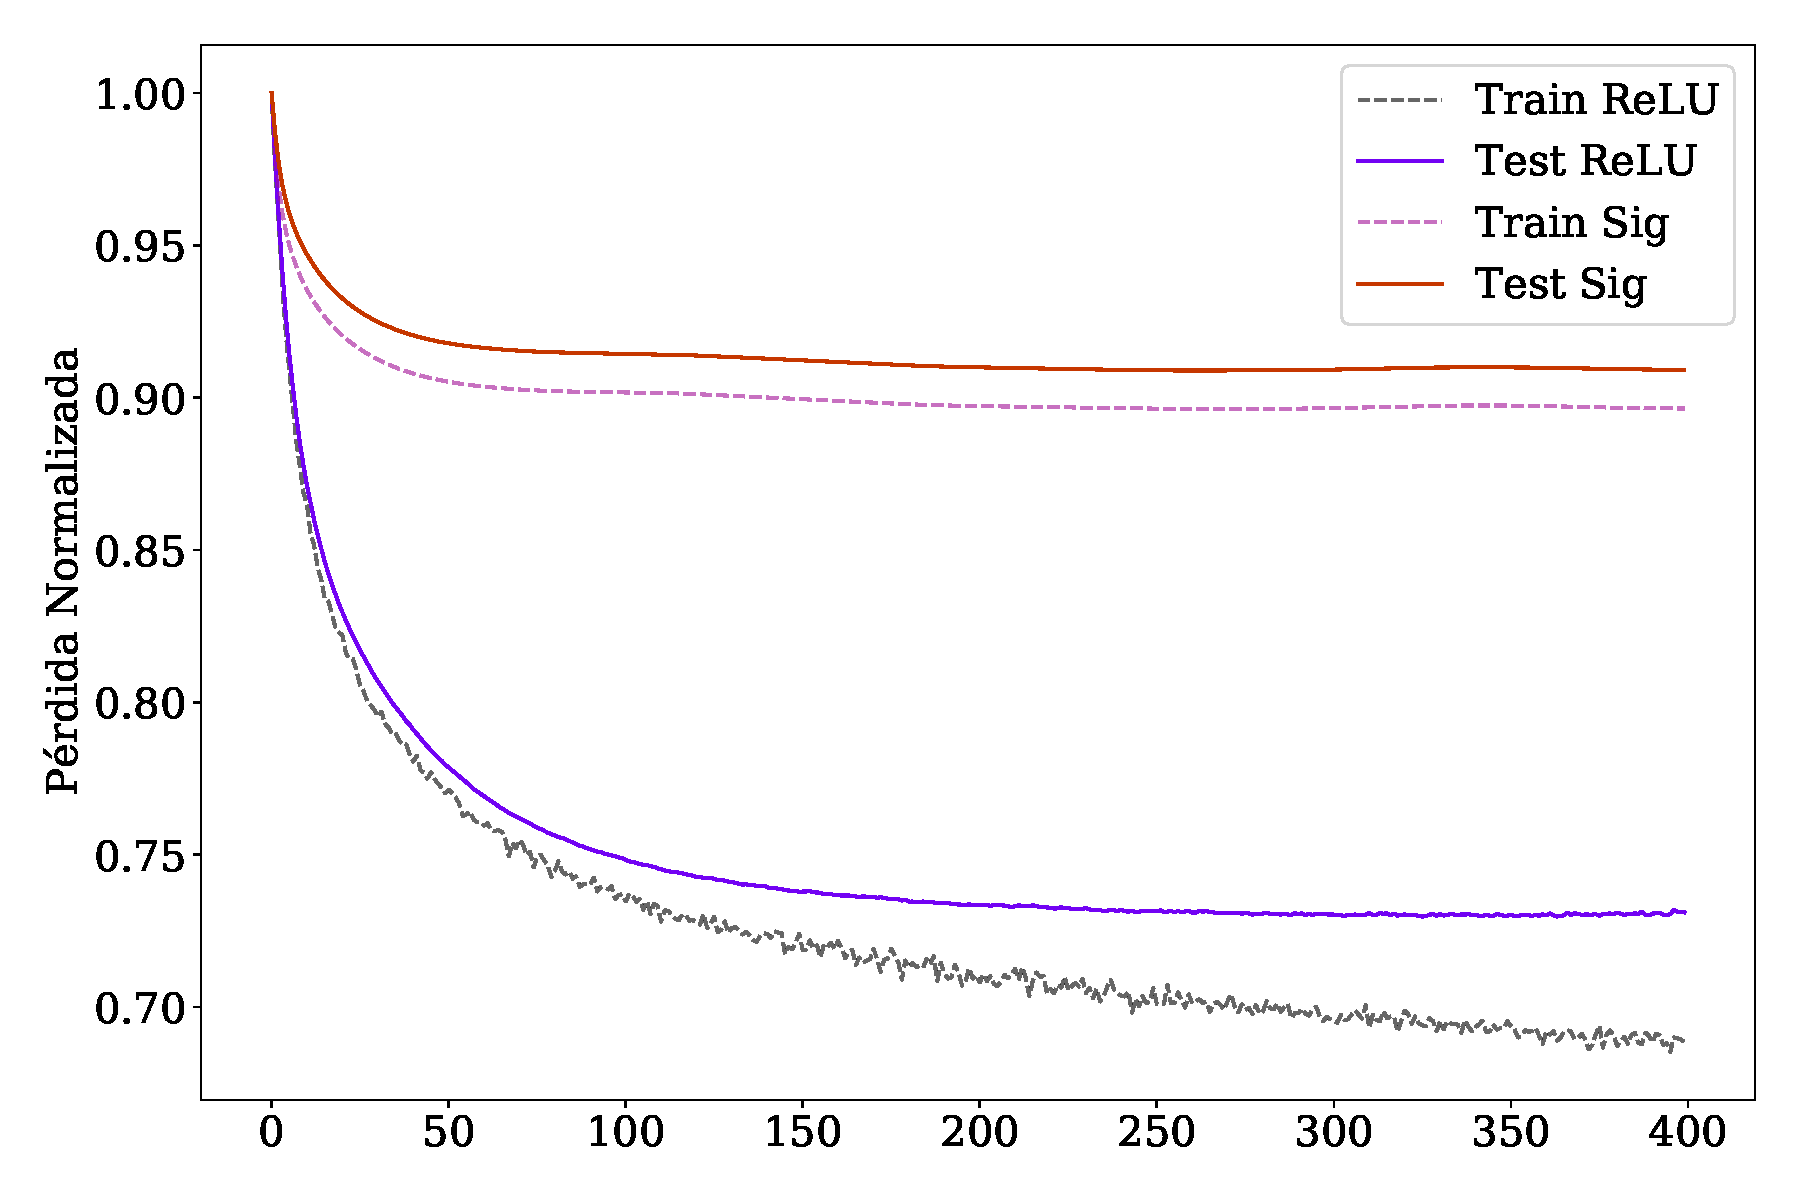
\includegraphics[width=0.465\textwidth]{Graphs/ejer8_loss.pdf}
        \end{center}
        \caption{Pérdida del entrenamiento  y validación  en función de las épocas para las dos redes implementadas en el ejercicio 8.}
        \label{fig:ejer8_loss}
    \end{small}
\end{figure}


\begin{figure}[H]
    \begin{small}
        \begin{center}
            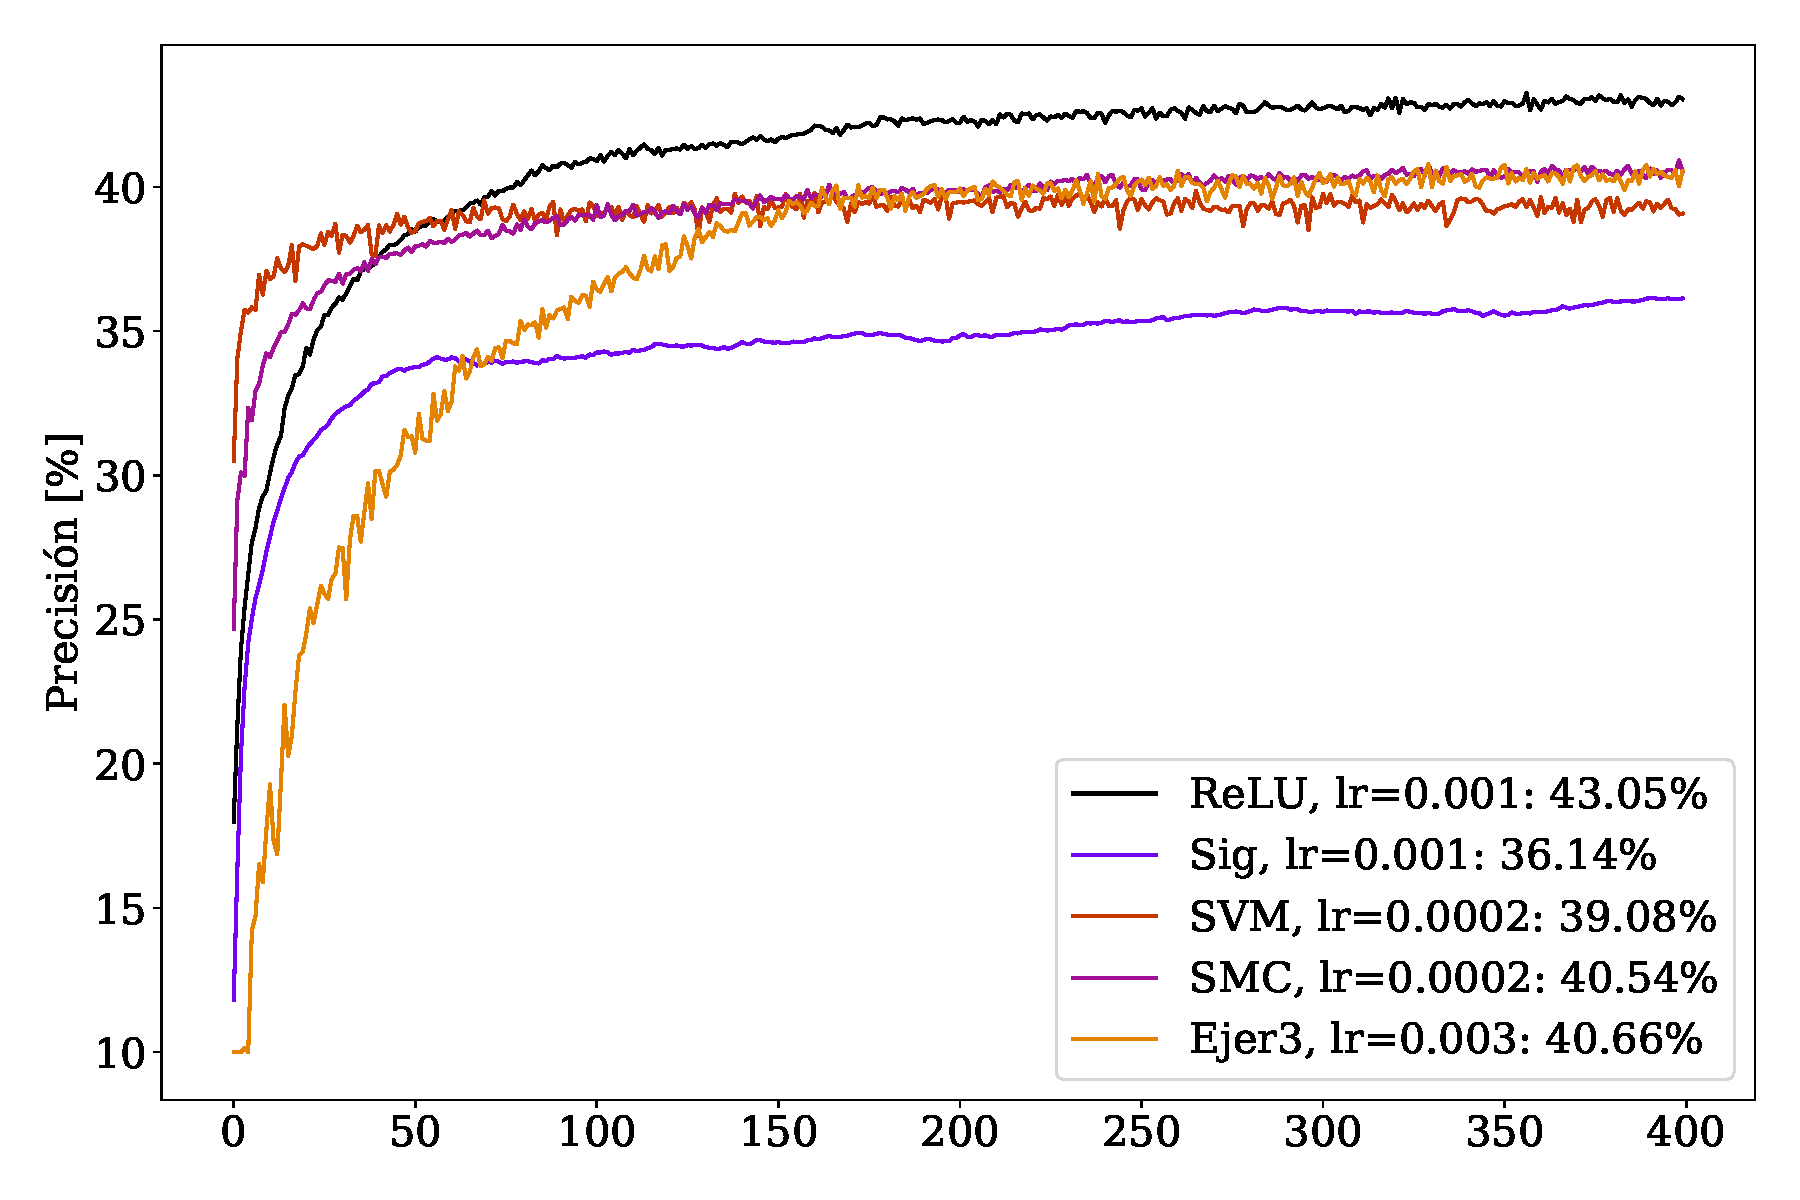
\includegraphics[width=0.465\textwidth]{Graphs/ejer8_acc_all.pdf}
        \end{center}
        \caption{Comparación de las precisiones de la conjunto de validación entre el ejercicio 8 y los clasificadores Soft-Max y Support Vector Machine de la práctica anterior.}
        \label{fig:ejer8_acc_all}
    \end{small}
\end{figure}

\end{document}